\documentclass{article}\usepackage[]{graphicx}\usepackage[]{color}
%% maxwidth is the original width if it is less than linewidth
%% otherwise use linewidth (to make sure the graphics do not exceed the margin)
\makeatletter
\def\maxwidth{ %
  \ifdim\Gin@nat@width>\linewidth
    \linewidth
  \else
    \Gin@nat@width
  \fi
}
\makeatother

\definecolor{fgcolor}{rgb}{0.345, 0.345, 0.345}
\newcommand{\hlnum}[1]{\textcolor[rgb]{0.686,0.059,0.569}{#1}}%
\newcommand{\hlstr}[1]{\textcolor[rgb]{0.192,0.494,0.8}{#1}}%
\newcommand{\hlcom}[1]{\textcolor[rgb]{0.678,0.584,0.686}{\textit{#1}}}%
\newcommand{\hlopt}[1]{\textcolor[rgb]{0,0,0}{#1}}%
\newcommand{\hlstd}[1]{\textcolor[rgb]{0.345,0.345,0.345}{#1}}%
\newcommand{\hlkwa}[1]{\textcolor[rgb]{0.161,0.373,0.58}{\textbf{#1}}}%
\newcommand{\hlkwb}[1]{\textcolor[rgb]{0.69,0.353,0.396}{#1}}%
\newcommand{\hlkwc}[1]{\textcolor[rgb]{0.333,0.667,0.333}{#1}}%
\newcommand{\hlkwd}[1]{\textcolor[rgb]{0.737,0.353,0.396}{\textbf{#1}}}%
\let\hlipl\hlkwb

\usepackage{framed}
\makeatletter
\newenvironment{kframe}{%
 \def\at@end@of@kframe{}%
 \ifinner\ifhmode%
  \def\at@end@of@kframe{\end{minipage}}%
  \begin{minipage}{\columnwidth}%
 \fi\fi%
 \def\FrameCommand##1{\hskip\@totalleftmargin \hskip-\fboxsep
 \colorbox{shadecolor}{##1}\hskip-\fboxsep
     % There is no \\@totalrightmargin, so:
     \hskip-\linewidth \hskip-\@totalleftmargin \hskip\columnwidth}%
 \MakeFramed {\advance\hsize-\width
   \@totalleftmargin\z@ \linewidth\hsize
   \@setminipage}}%
 {\par\unskip\endMakeFramed%
 \at@end@of@kframe}
\makeatother

\definecolor{shadecolor}{rgb}{.97, .97, .97}
\definecolor{messagecolor}{rgb}{0, 0, 0}
\definecolor{warningcolor}{rgb}{1, 0, 1}
\definecolor{errorcolor}{rgb}{1, 0, 0}
\newenvironment{knitrout}{}{} % an empty environment to be redefined in TeX

\usepackage{alltt}
\usepackage[utf8]{inputenc}
\usepackage{hyperref}
\hypersetup{
    linktocpage,
    colorlinks=true, 
    linkcolor=blue,
    citecolor=blue,
    filecolor=blue,
    urlcolor=blue
}
\IfFileExists{upquote.sty}{\usepackage{upquote}}{}
\begin{document}


\title{Transcription vs Metilation}
\author{Lucas Michel Todó}
\maketitle
\tableofcontents
\clearpage

%------------------------------------------------------------------------------------------------------------------------------------------
%---------------------------------------------------------INTRO----------------------------------------------------------------------------


\section{Generalitats}
En TOTS els gràfics la columna de més a l'esquerra correspon als valors de diferència de transcripció (1.2B - 10G). Les columnes següents corresponen a algun paràmetre relacionat amb la metilació (percentatge del gen metilat, coverage mitjà...). En alguns casos hi ha valor de metilació per a 1.2B i per a 10G i en altres una sola columna que correspon a la diferència de metilació. Per a cada tipus de gràfic se n'han fet diversos tenint en compte la metilació a tres zones diferents: TSS, gene-body i TTS. Per a cada tipus de gràfic he posat el més representatiu a tall d'exemple. Al final del document hi ha tota la resta de gràfics.
\clearpage

%------------------------------------------------------------------------------------------------------------------------------------------
%---------------------------------------------------------PERCENATGE-----------------------------------------------------------------------

\section{Heatmaps Percentatge de Coverage}
En aquest gràfics els valors corresponents a les columnes 1.2B i 10G corresponen al percentatge del gen cobert en pics diferencials. Per a obtenir aquests valors s'han unificat les dues llistes de pics differencials annotats. Tant per a 1.2B com a 10G els gens que corresponen a "pics de l'altra llista" tenen valors de 0.
\subsection{TSS+Gene+TTS}
\begin{knitrout}
\definecolor{shadecolor}{rgb}{0.969, 0.969, 0.969}\color{fgcolor}

{\centering 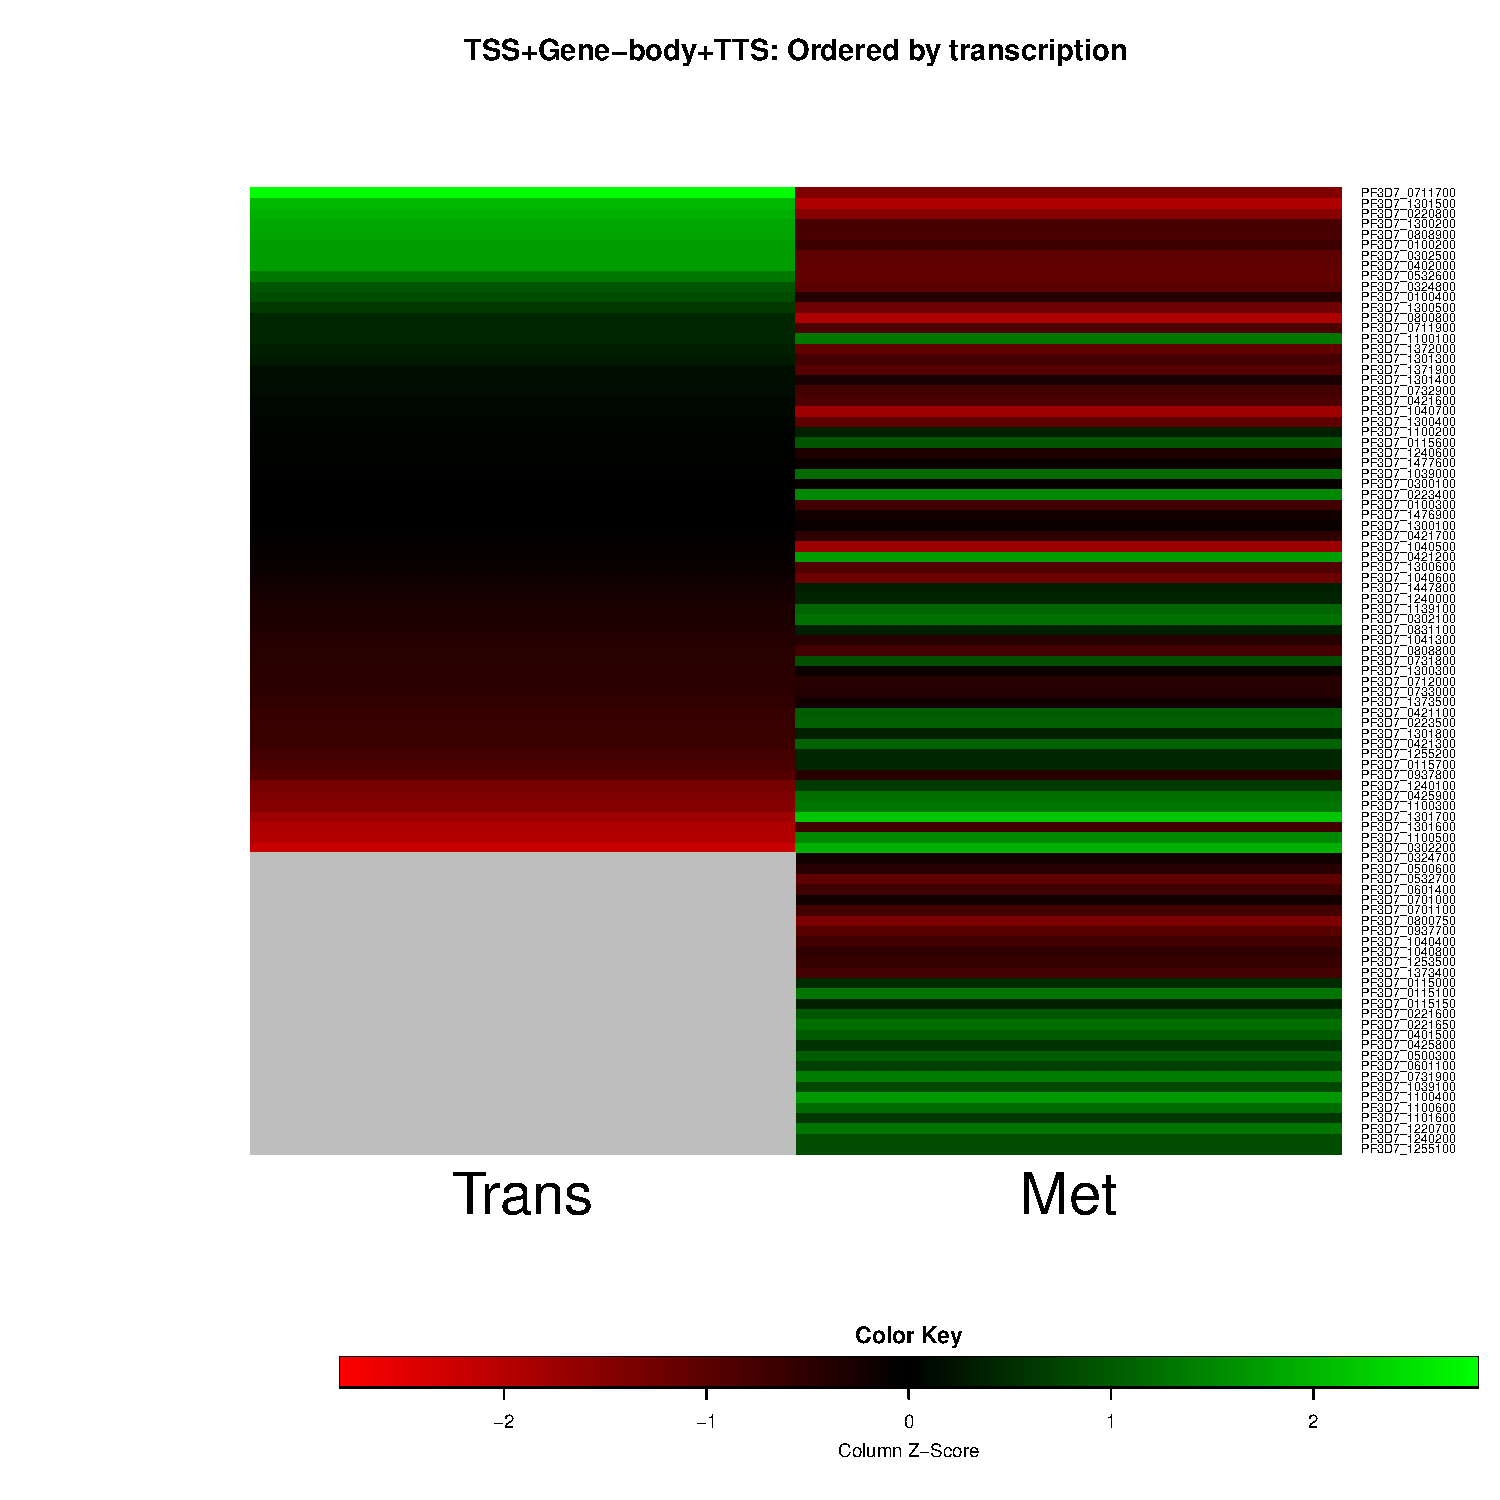
\includegraphics[width=.9\linewidth]{figure/minimal-heatmap_all-1} 

}



\end{knitrout}
\clearpage
\begin{knitrout}
\definecolor{shadecolor}{rgb}{0.969, 0.969, 0.969}\color{fgcolor}

{\centering 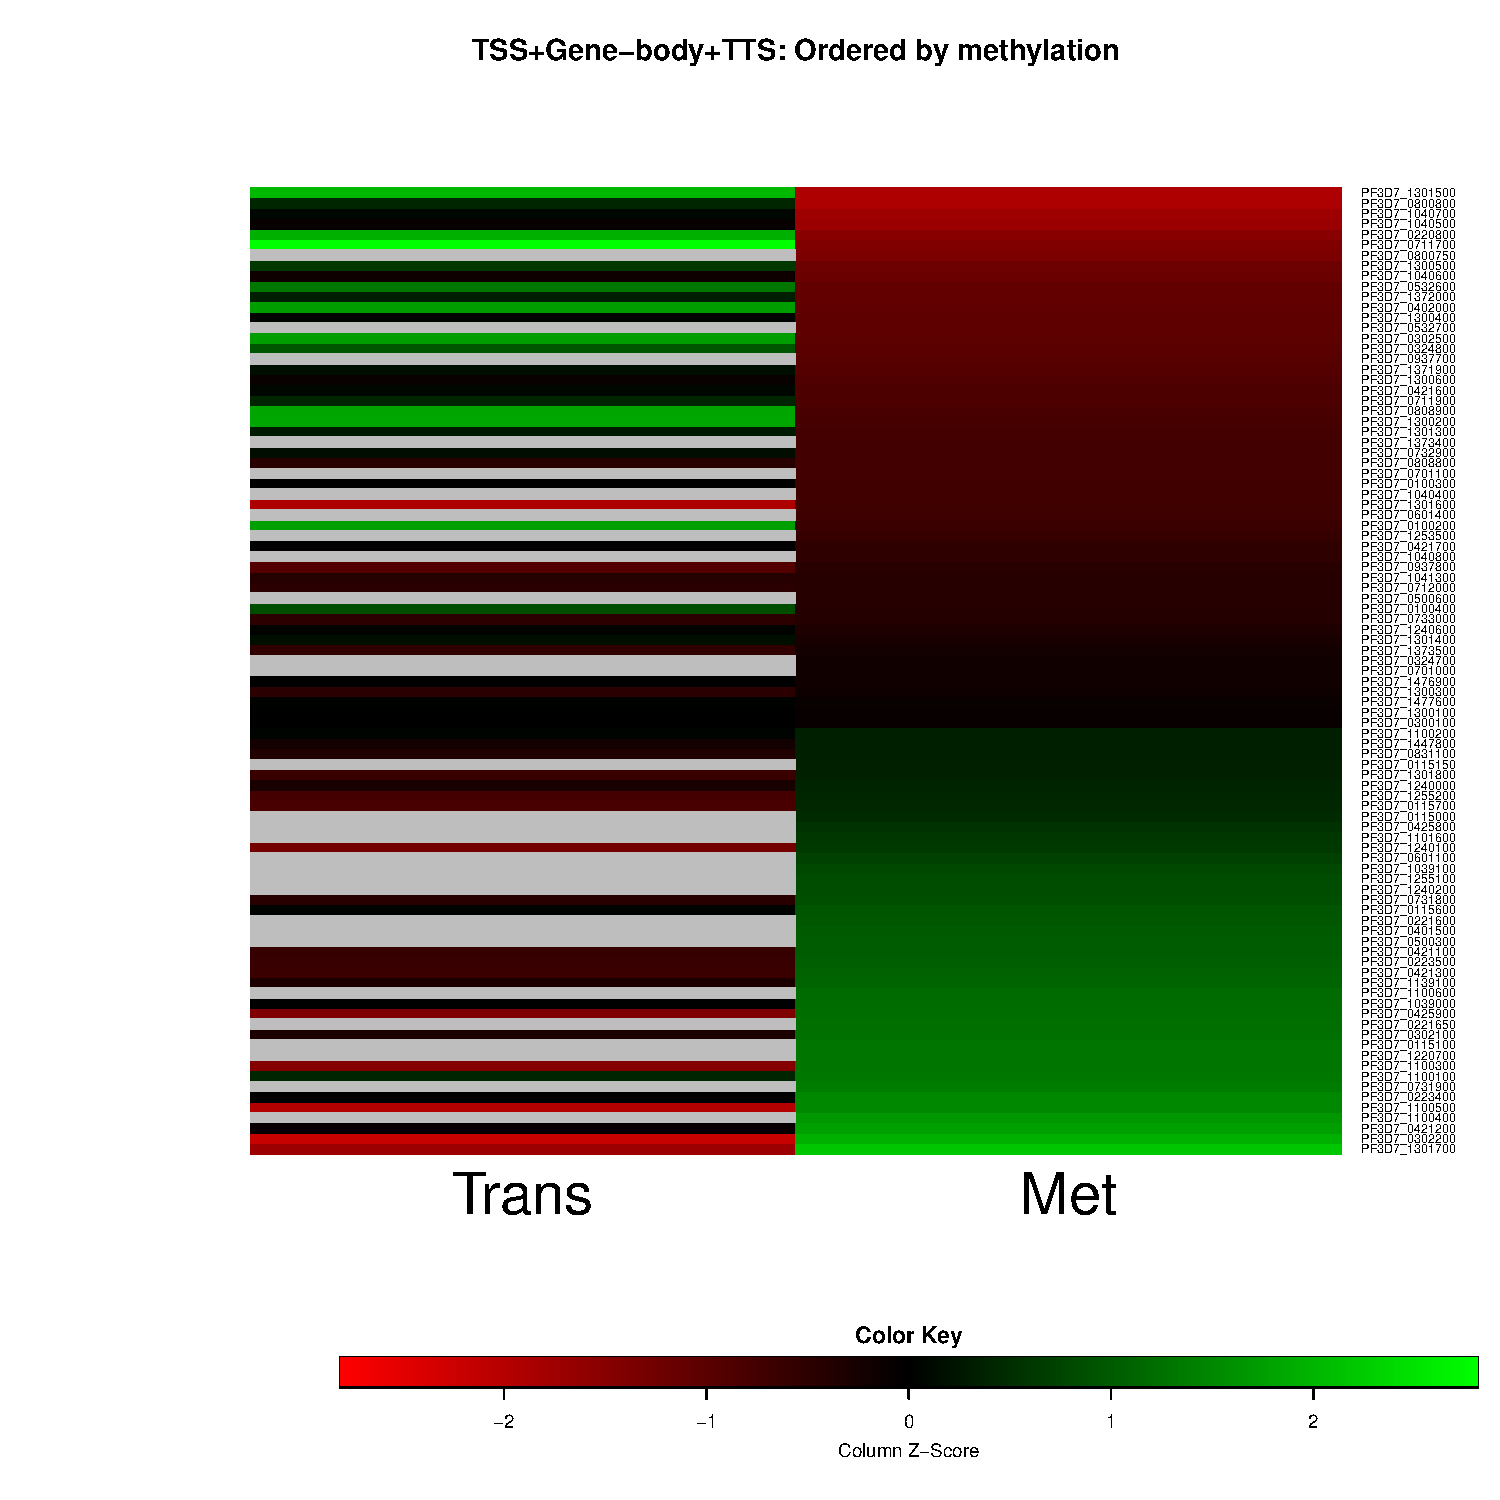
\includegraphics[width=.9\linewidth]{figure/minimal-heatmap_all_metord-1} 

}



\end{knitrout}

%------------------------------------------------------------------------------------------------------------------------------------------
%---------------------------------------------------------COVERAGE-------------------------------------------------------------------------
\clearpage
\section{Heatmaps Coverage}
En aquests gràfics el valors de les columnes 1.2B i 10G corresponen al valor de coverage de cada gen. El coverage s'ha calculat per a tots els gens i s'ha "normalitzat" tant per nombre de reads (per a compensar el fet que els alineaments amb més reads tenen més coverage en general) com pel tamany del gen (per compensar el fet que els gens més llargs tenen més reads). Els gens que es mostren al gràfic estàn filtrats: només apareixen aquells que tenen una diferència de transcripció (primera columna) major a 0.7 (en valor absolut).

\subsection{Coverage Gene Body + 5'}
\begin{knitrout}
\definecolor{shadecolor}{rgb}{0.969, 0.969, 0.969}\color{fgcolor}

{\centering 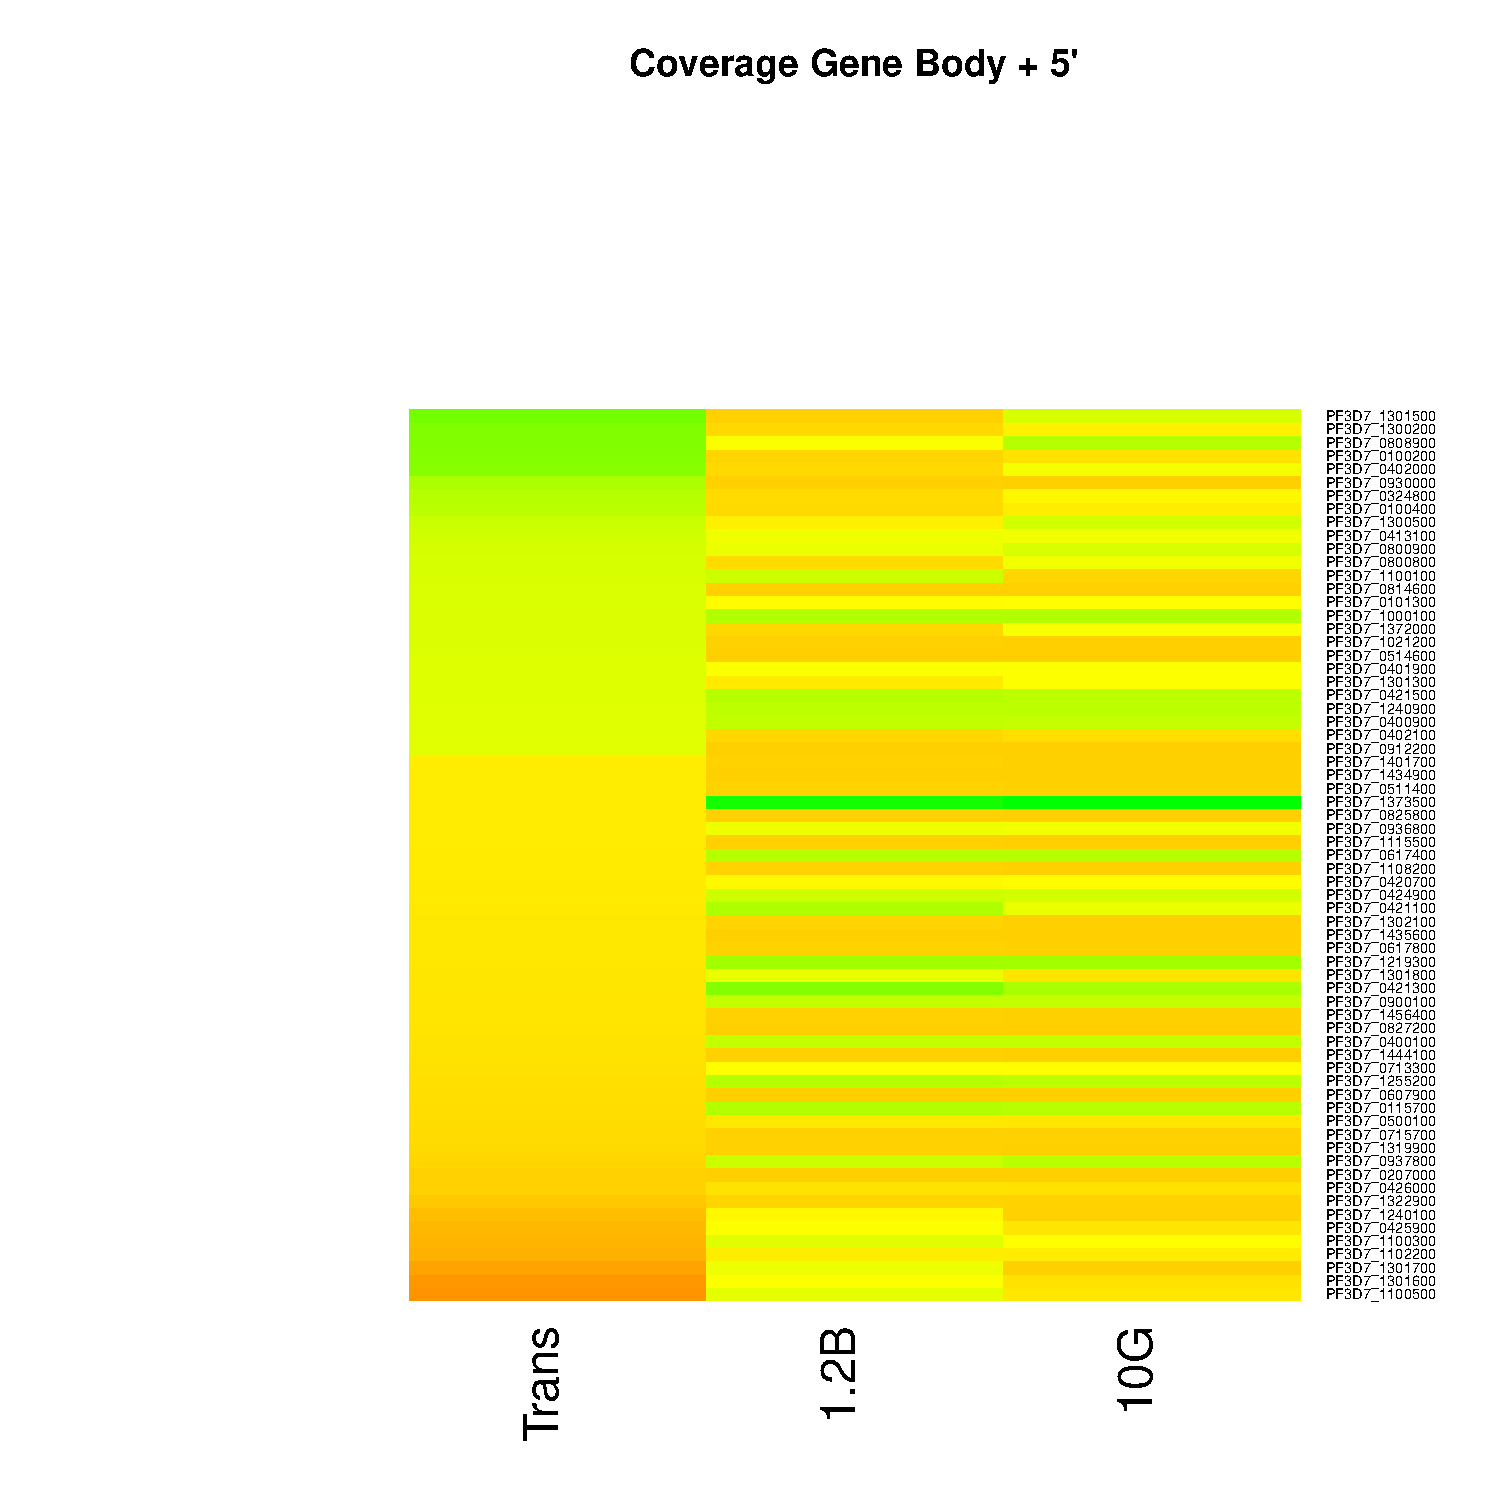
\includegraphics[width=.9\linewidth]{figure/minimal-heat_cov_tss_gene-1} 

}



\end{knitrout}
\clearpage

%------------------------------------------------------------------------------------------------------------------------------------------
%---------------------------------------------------------DIFERÈNCIA DE COVERAGE-----------------------------------------------------------

\subsection{Diferència de Coverage, filtrat per diferència de transcripció}
En aquests gràfics hi ha una sola columna corresponent a metilació que correspon a diferència de coverage. Aquesta diferència és simplement la resta (1.2B - 10G) dels valors obtinguts en l'apartat anterior.
\begin{knitrout}
\definecolor{shadecolor}{rgb}{0.969, 0.969, 0.969}\color{fgcolor}

{\centering 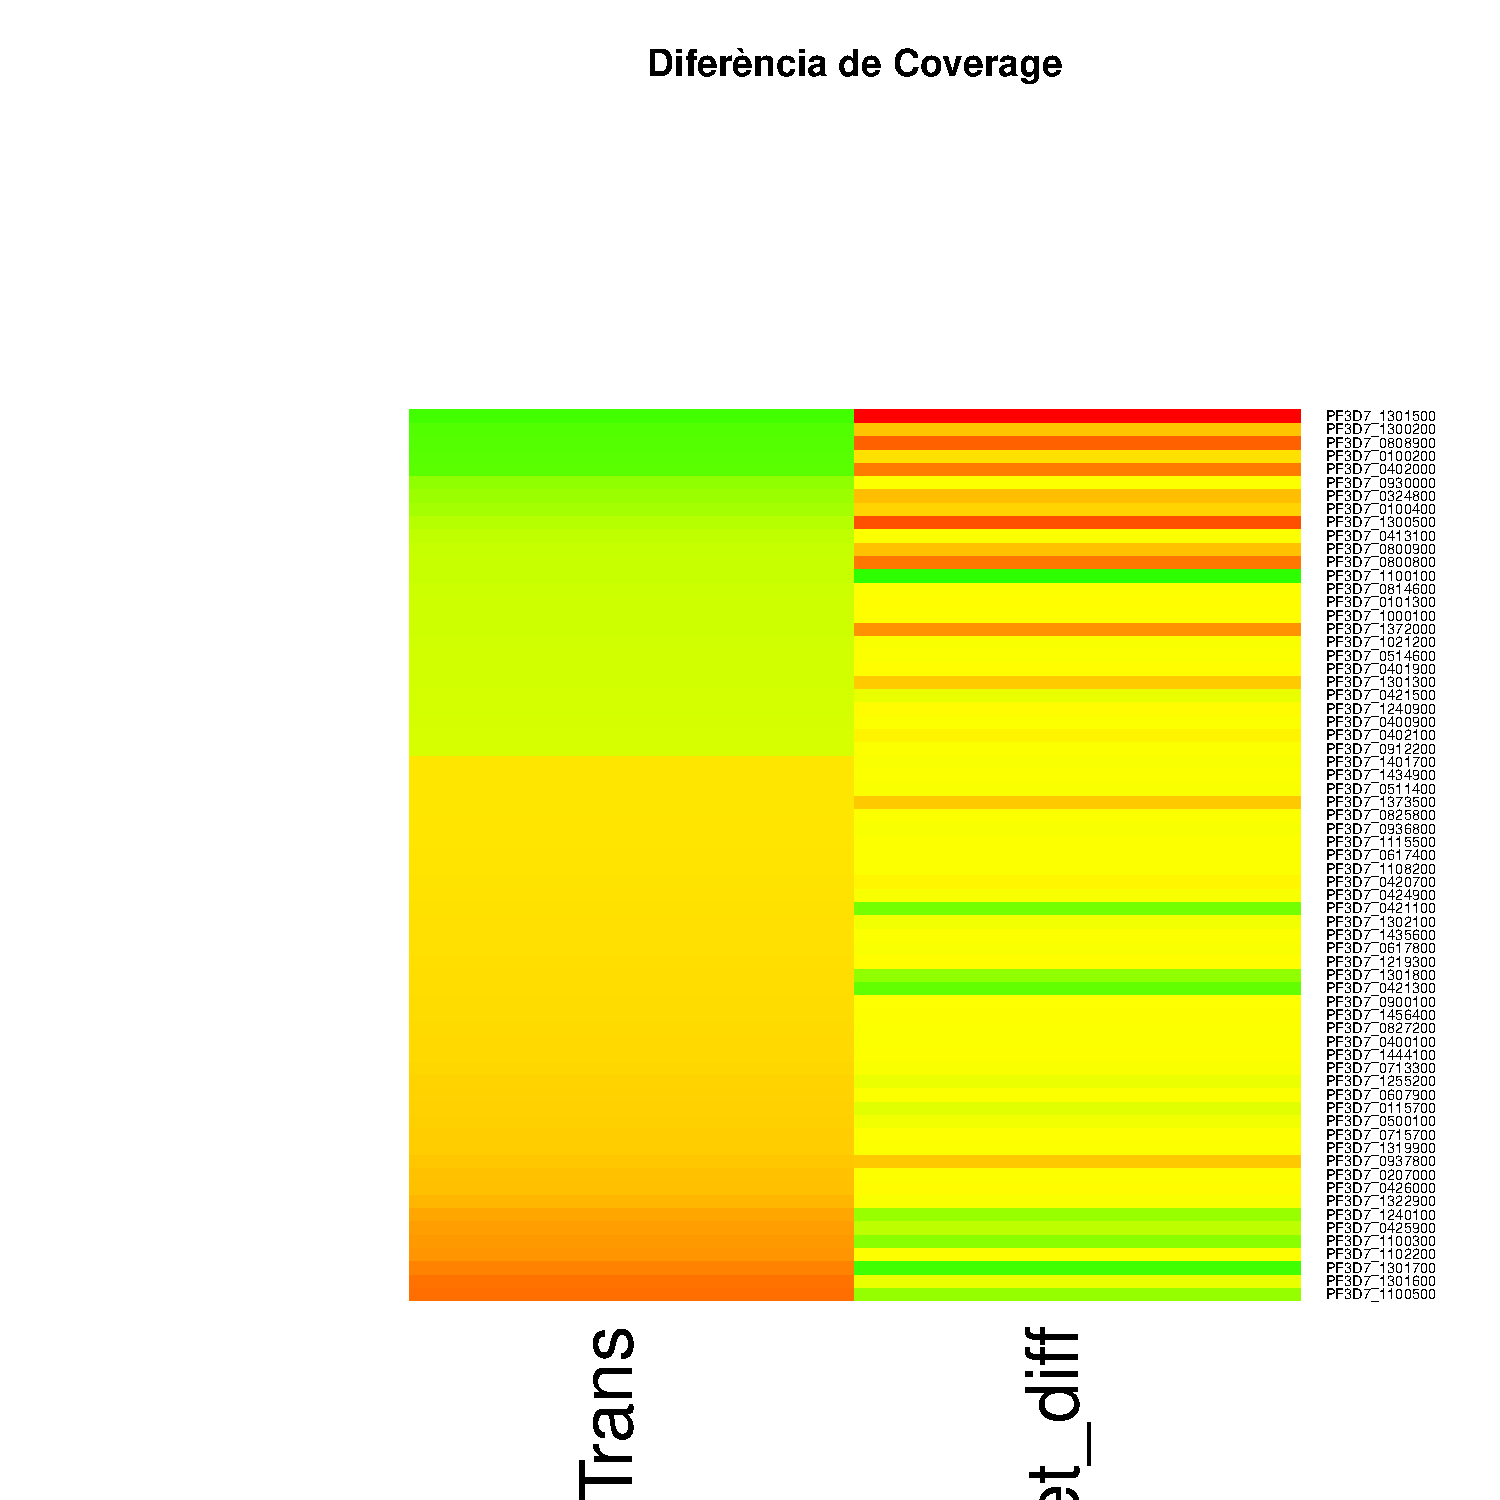
\includegraphics[width=.9\linewidth]{figure/minimal-_heat_cov_diff-1} 

}



\end{knitrout}
\clearpage
\begin{knitrout}
\definecolor{shadecolor}{rgb}{0.969, 0.969, 0.969}\color{fgcolor}

{\centering 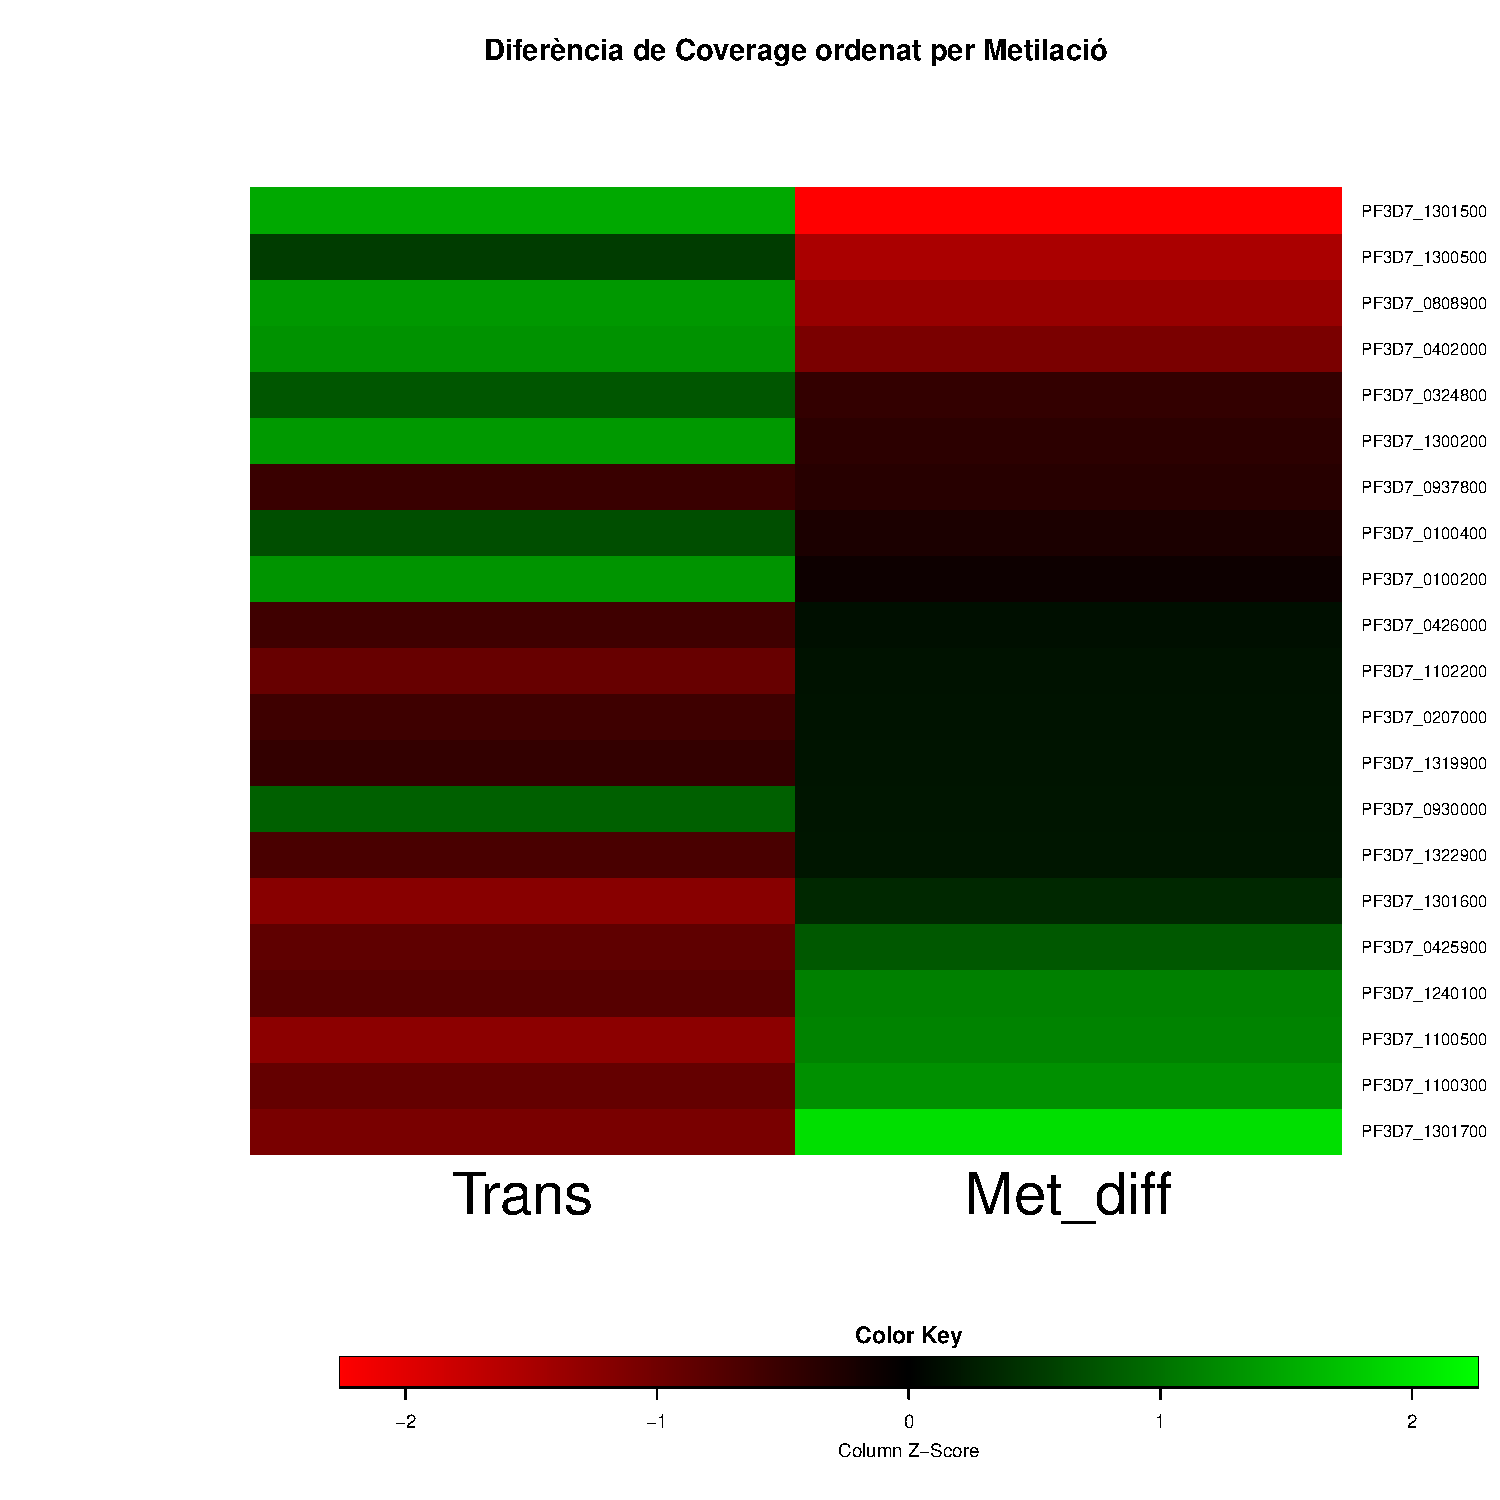
\includegraphics[width=.9\linewidth]{figure/minimal-_heat_cov_diff_metord-1} 

}



\end{knitrout}
\clearpage
\subsection{Diferència de Coverage, filtrat per diferència de metilació}
Aquest gràfic és el mateix que l'anterior però en comptes de filtrar per valors de transcripció els gens que hi apareixen estàn filtrats per valors de metilació. Els gens que apreixen al gràfic són aquells què apareixen a alguna de les llistes de gens pics diferencials.
\begin{knitrout}
\definecolor{shadecolor}{rgb}{0.969, 0.969, 0.969}\color{fgcolor}

{\centering 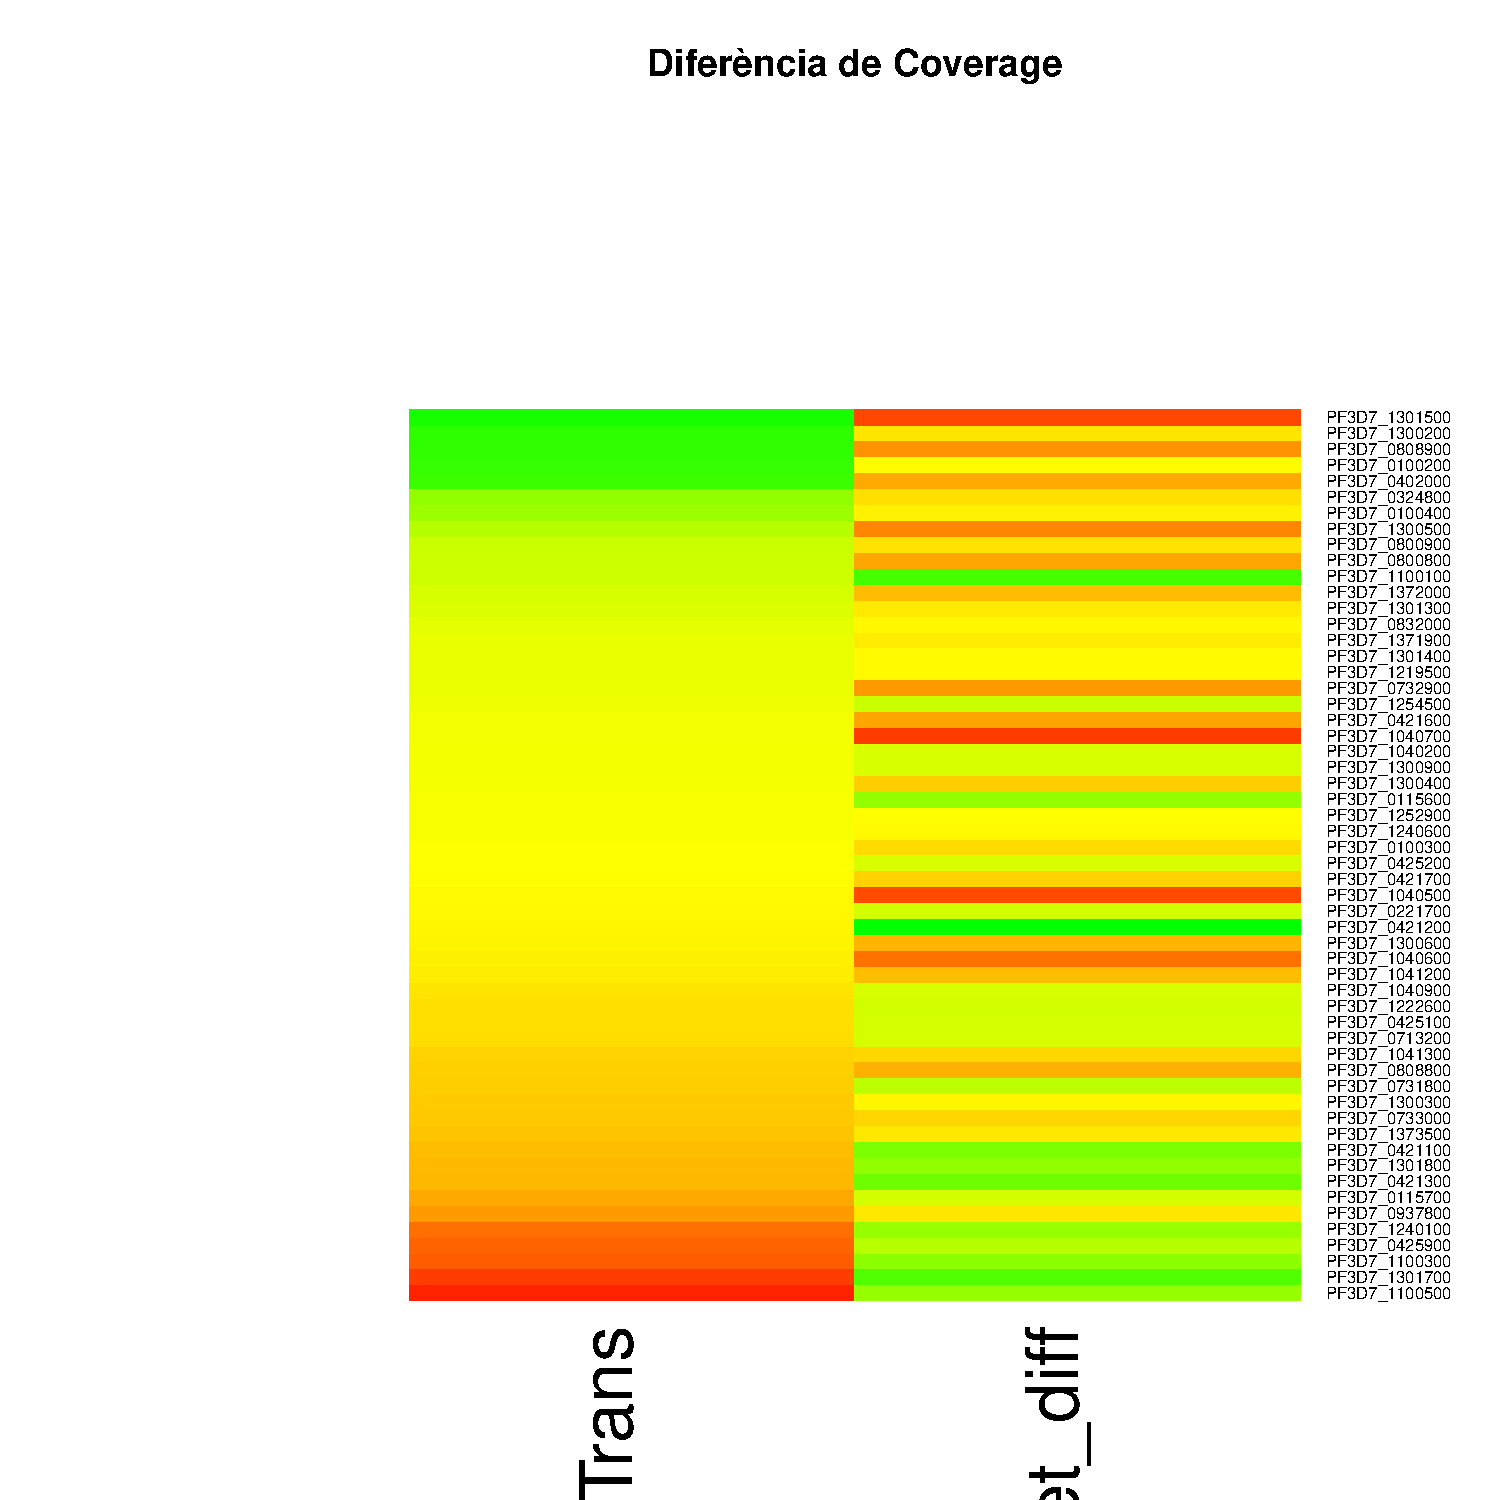
\includegraphics[width=.9\linewidth]{figure/minimal-heat_cov_diff_filter-1} 

}



\end{knitrout}
\clearpage
En aquest cas hem deixat els gens per als que no tenim valors de transcripció.
\begin{knitrout}
\definecolor{shadecolor}{rgb}{0.969, 0.969, 0.969}\color{fgcolor}

{\centering 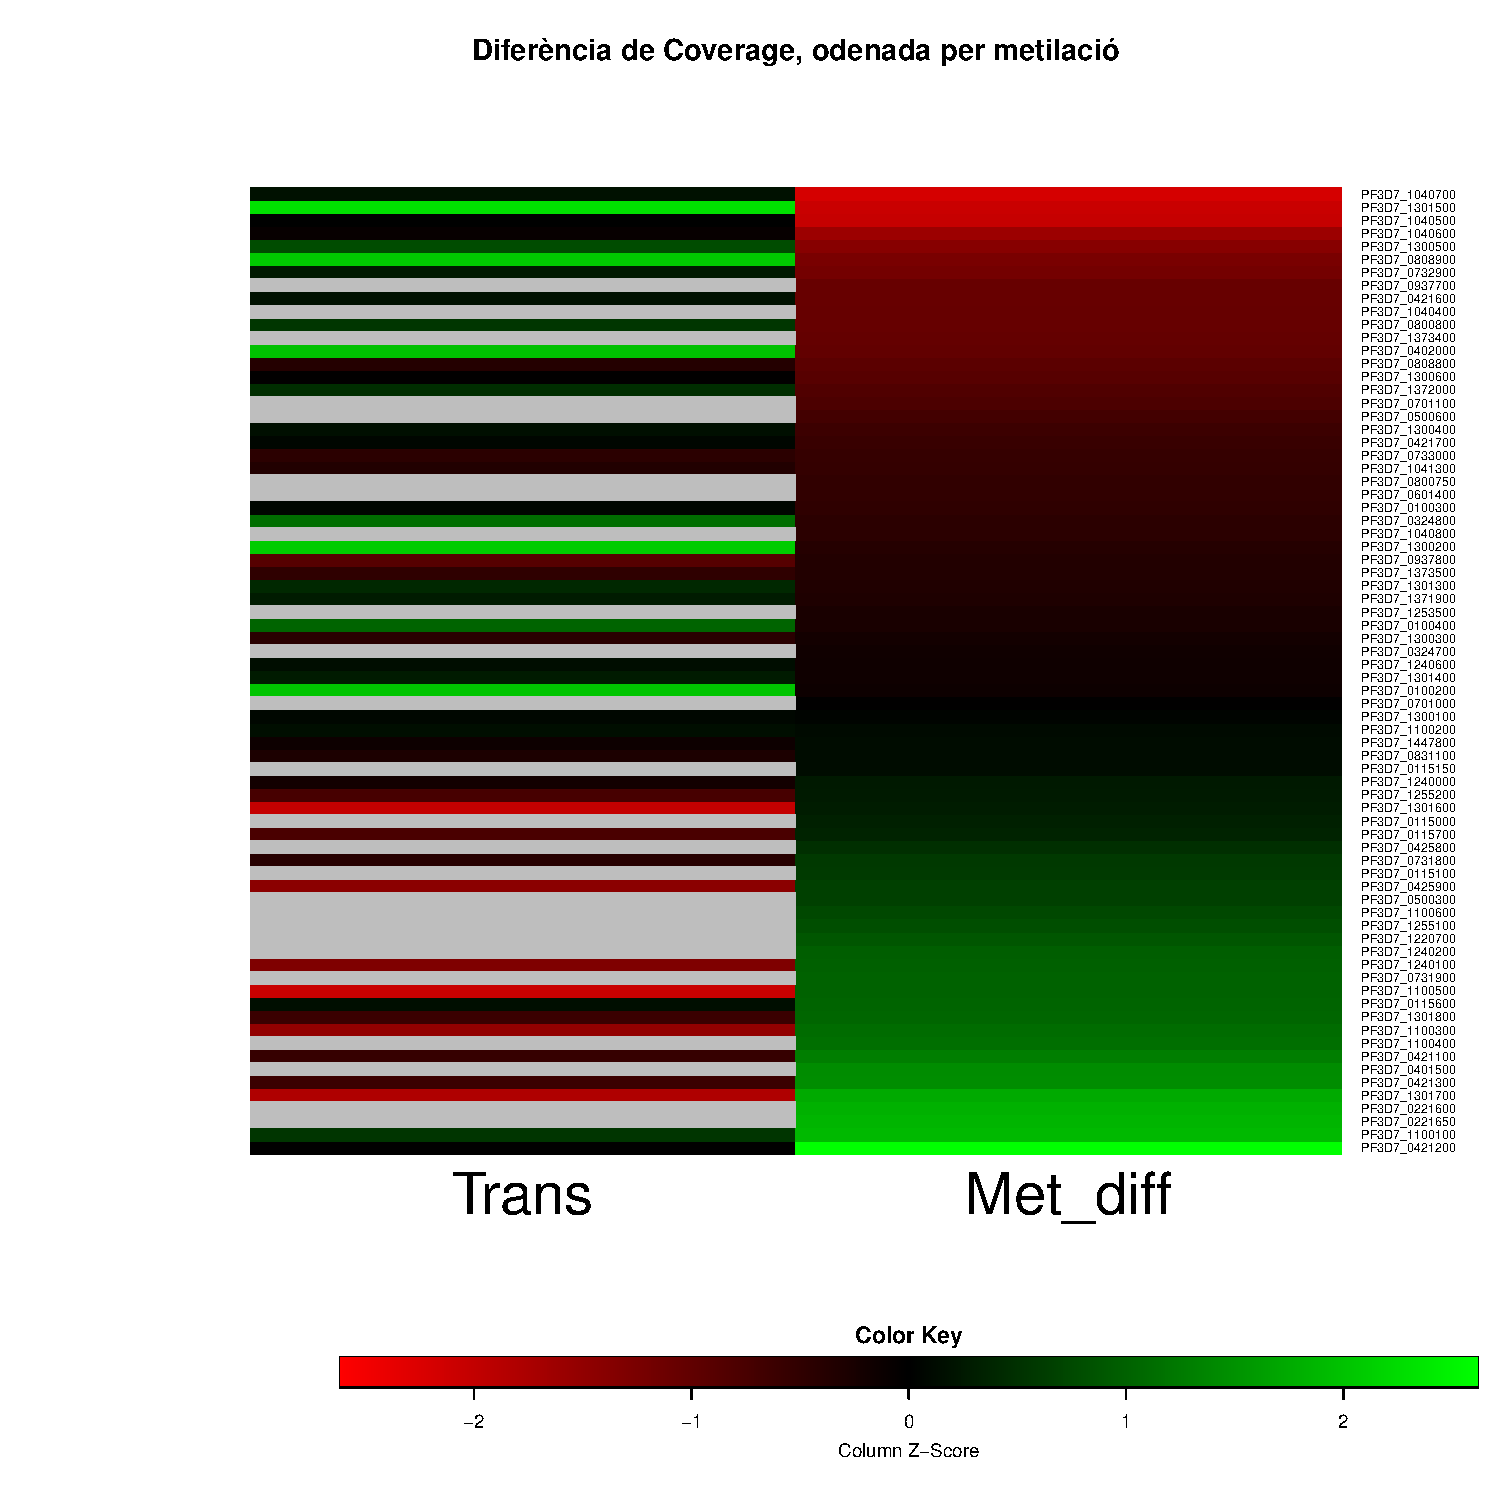
\includegraphics[width=.9\linewidth]{figure/minimal-heat_cov_diff_filter_metord-1} 

}



\end{knitrout}
\clearpage
\subsection{Diferència de Coverage: auto-clustering}
En aquest cas hem deixat que els gens s'ordeni "sol" fent servir l'algoritme de clustering de la funció "heatmap2" d'R.
\begin{knitrout}
\definecolor{shadecolor}{rgb}{0.969, 0.969, 0.969}\color{fgcolor}

{\centering 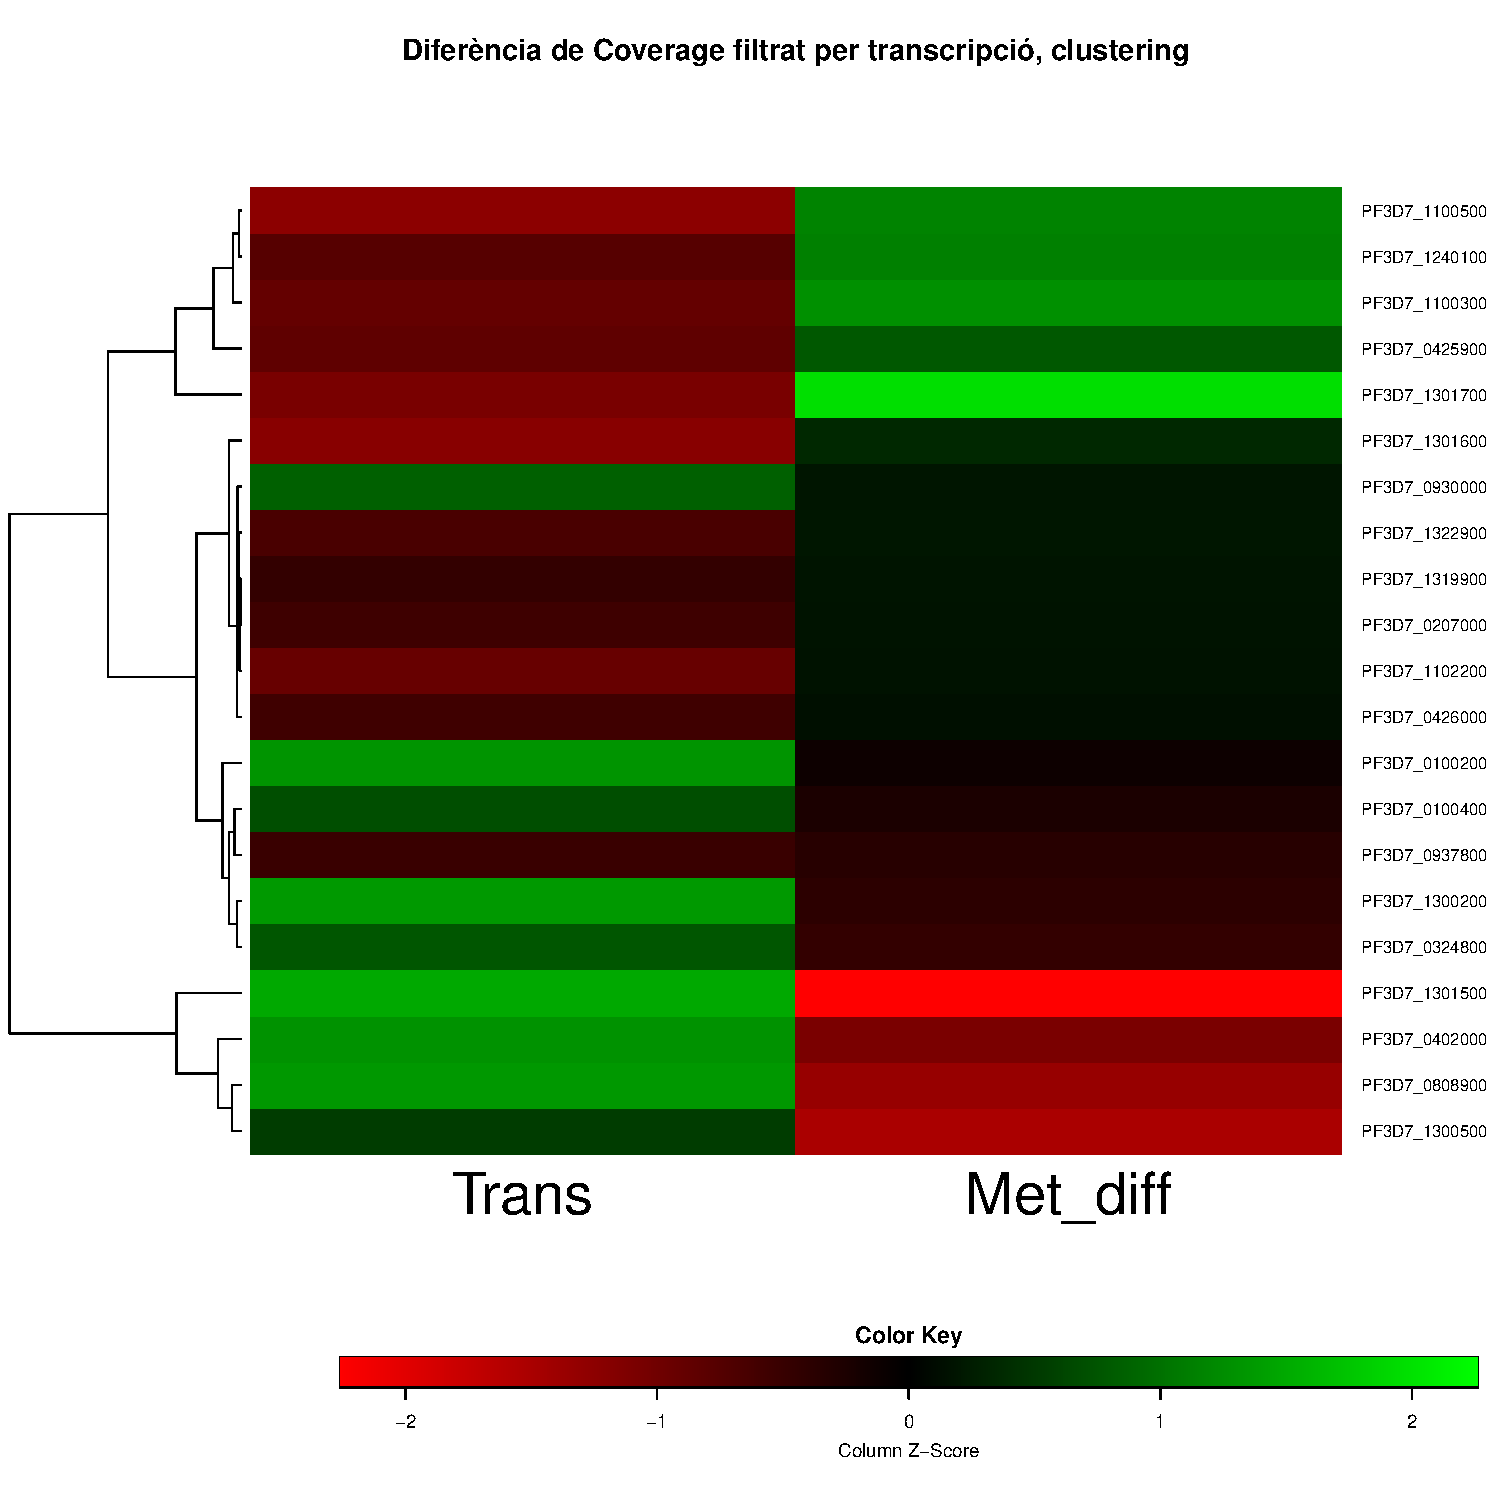
\includegraphics[width=.9\linewidth]{figure/minimal-heat_cov_diff_filter_cluster-1} 

}



\end{knitrout}
\clearpage
\begin{knitrout}
\definecolor{shadecolor}{rgb}{0.969, 0.969, 0.969}\color{fgcolor}

{\centering 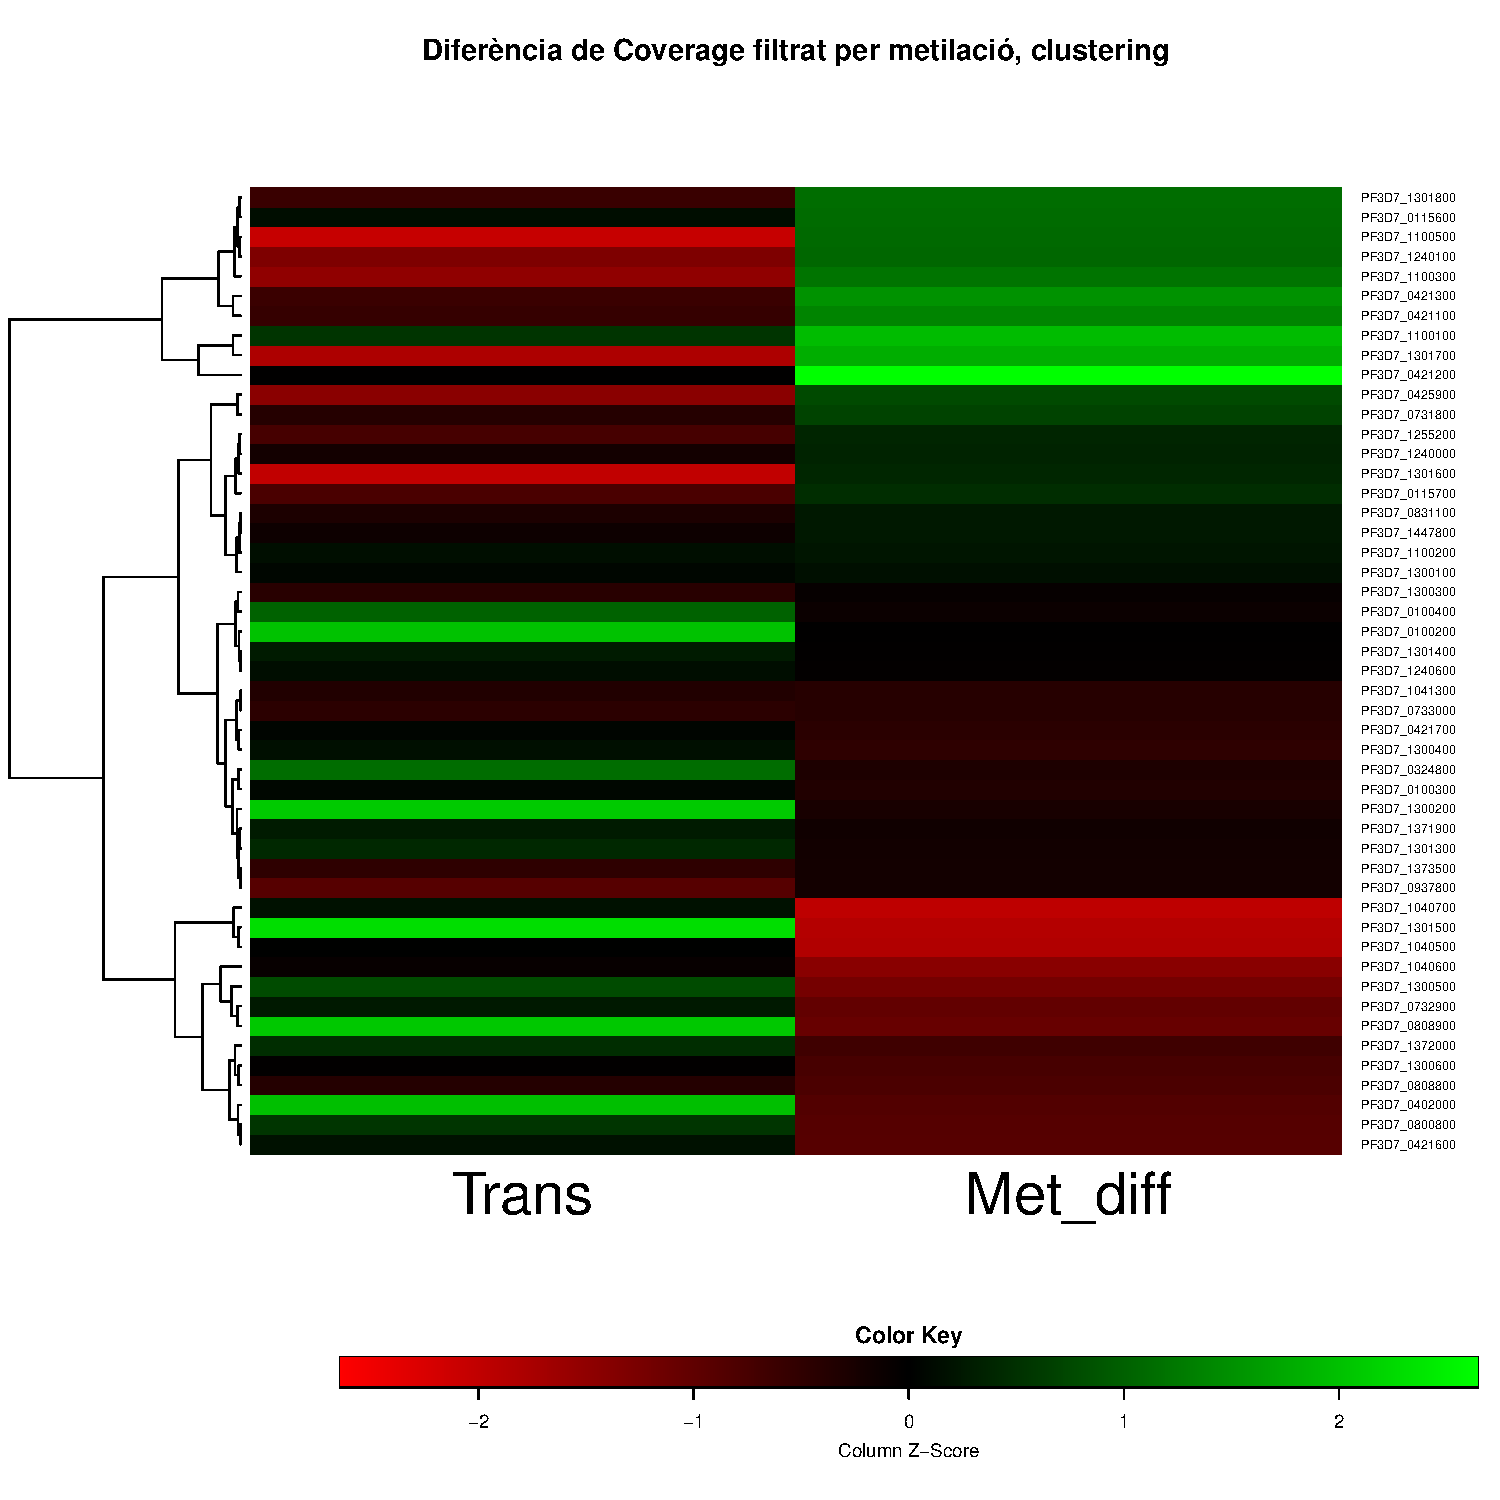
\includegraphics[width=.9\linewidth]{figure/minimal-heat_cov_met_filter_cluster-1} 

}



\end{knitrout}
%------------------------------------------------------------------------------------------------------------------------------------------
%---------------------------------------------------------COVERAGE A PICS DIFERENCIALS-----------------------------------------------------

\clearpage
\section{Coverage a pics diferencials}
En aquests gràfics s'ha calculat el coverage mitjà de la mateixa manera que en els anteriors, però l'anàlisi s'ha restringit a aquells gens que apareixen a qualsevol de les dues llistes de pics diferencials (pics diferencials a 1.2B i a 10G). 

\subsection{Coverage a pics diferencials}
En aquests gràfics els valors de les columnes 1.2B i 10G corresponen al coverage mitjà de cada gen només a les zones on hi ha pics diferencials (de metilació).
\begin{knitrout}
\definecolor{shadecolor}{rgb}{0.969, 0.969, 0.969}\color{fgcolor}

{\centering 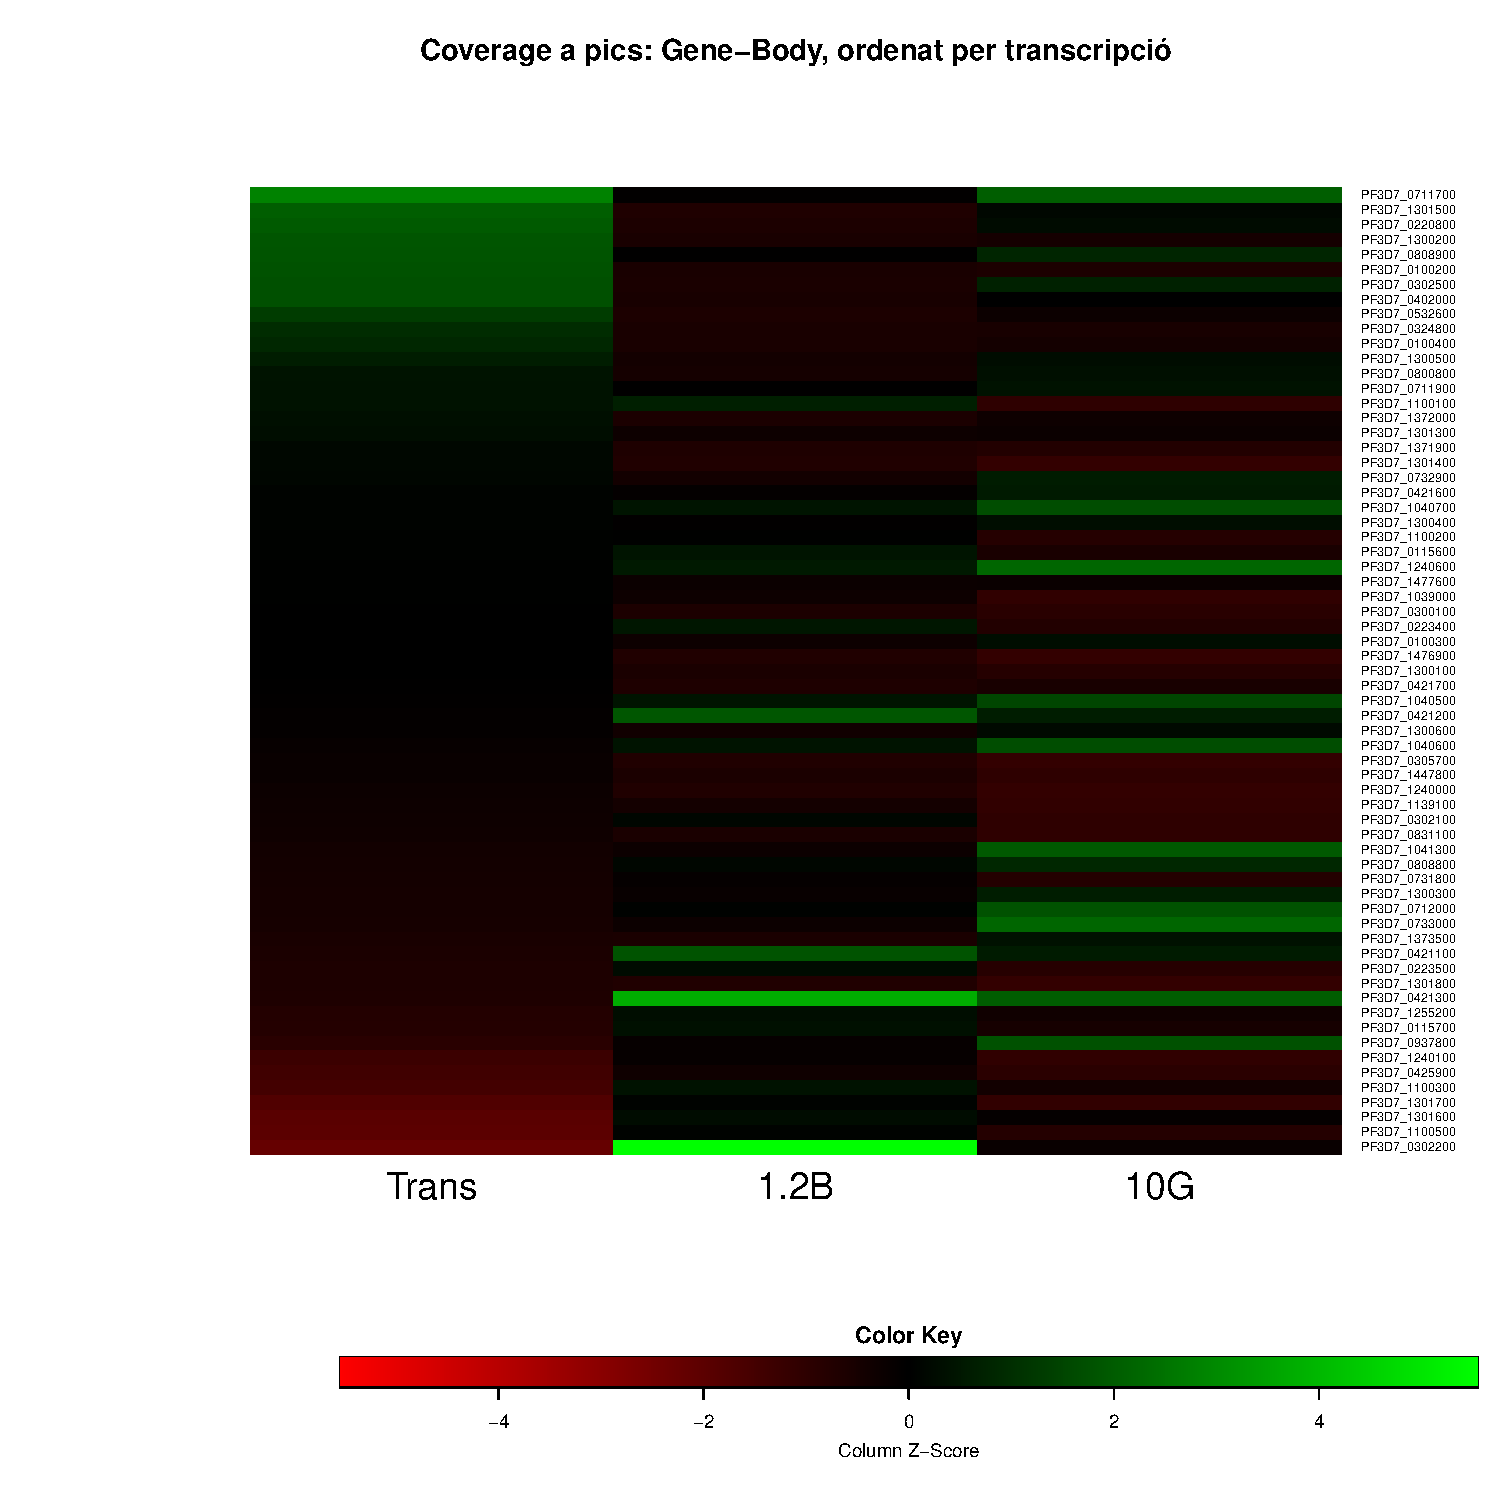
\includegraphics[width=.9\linewidth]{figure/minimal-heat_difpeak_cov-1} 

}



\end{knitrout}
\clearpage
\subsection{Diferència de coverage a pics diferencials}
En aquests gràfics tenim una sola columna a la dreta que correspon a la diferència de coverage entre 1.2B i 10G només a les zones on hi ha pics.
\begin{knitrout}
\definecolor{shadecolor}{rgb}{0.969, 0.969, 0.969}\color{fgcolor}

{\centering 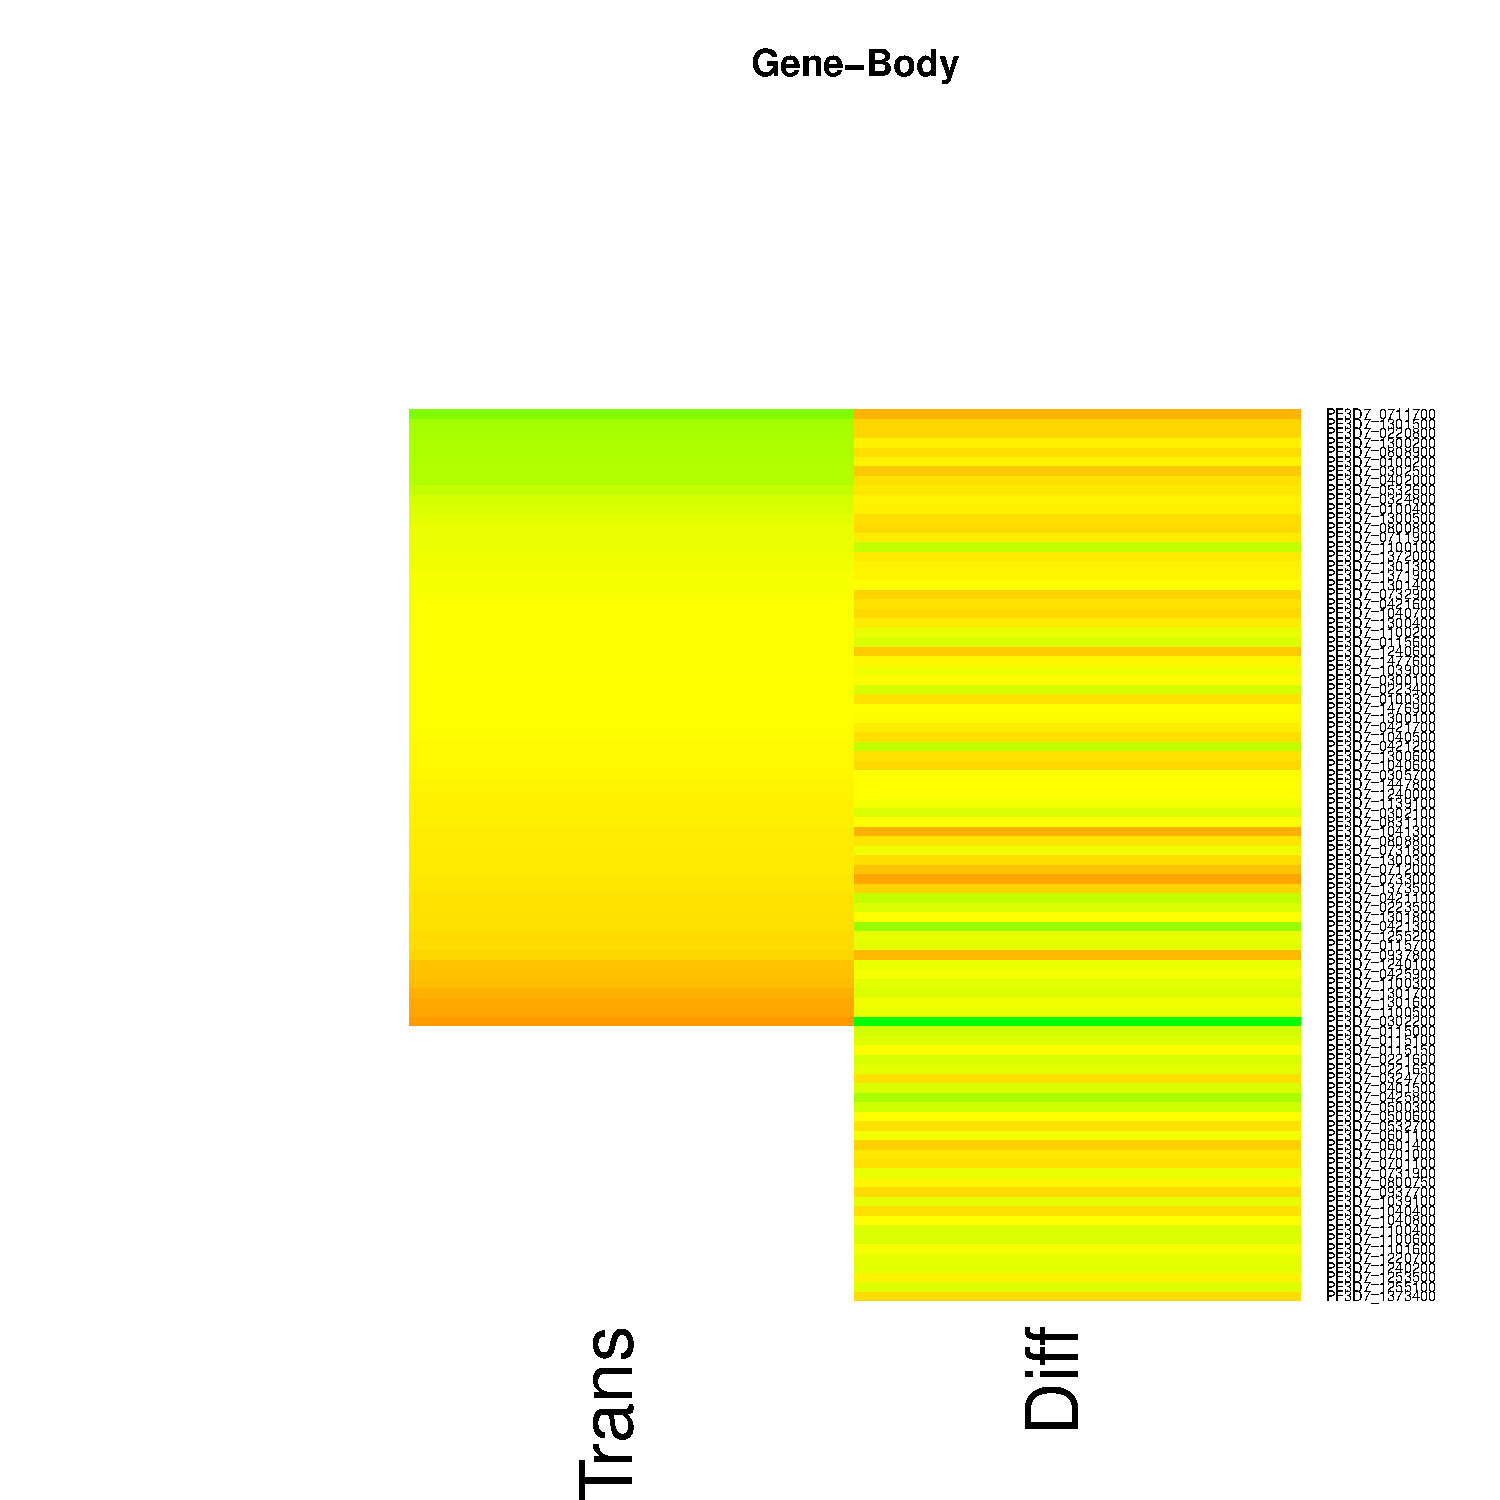
\includegraphics[width=.9\linewidth]{figure/minimal-heat_difpeak_cov_dif-1} 

}



\end{knitrout}
\clearpage
\begin{knitrout}
\definecolor{shadecolor}{rgb}{0.969, 0.969, 0.969}\color{fgcolor}

{\centering 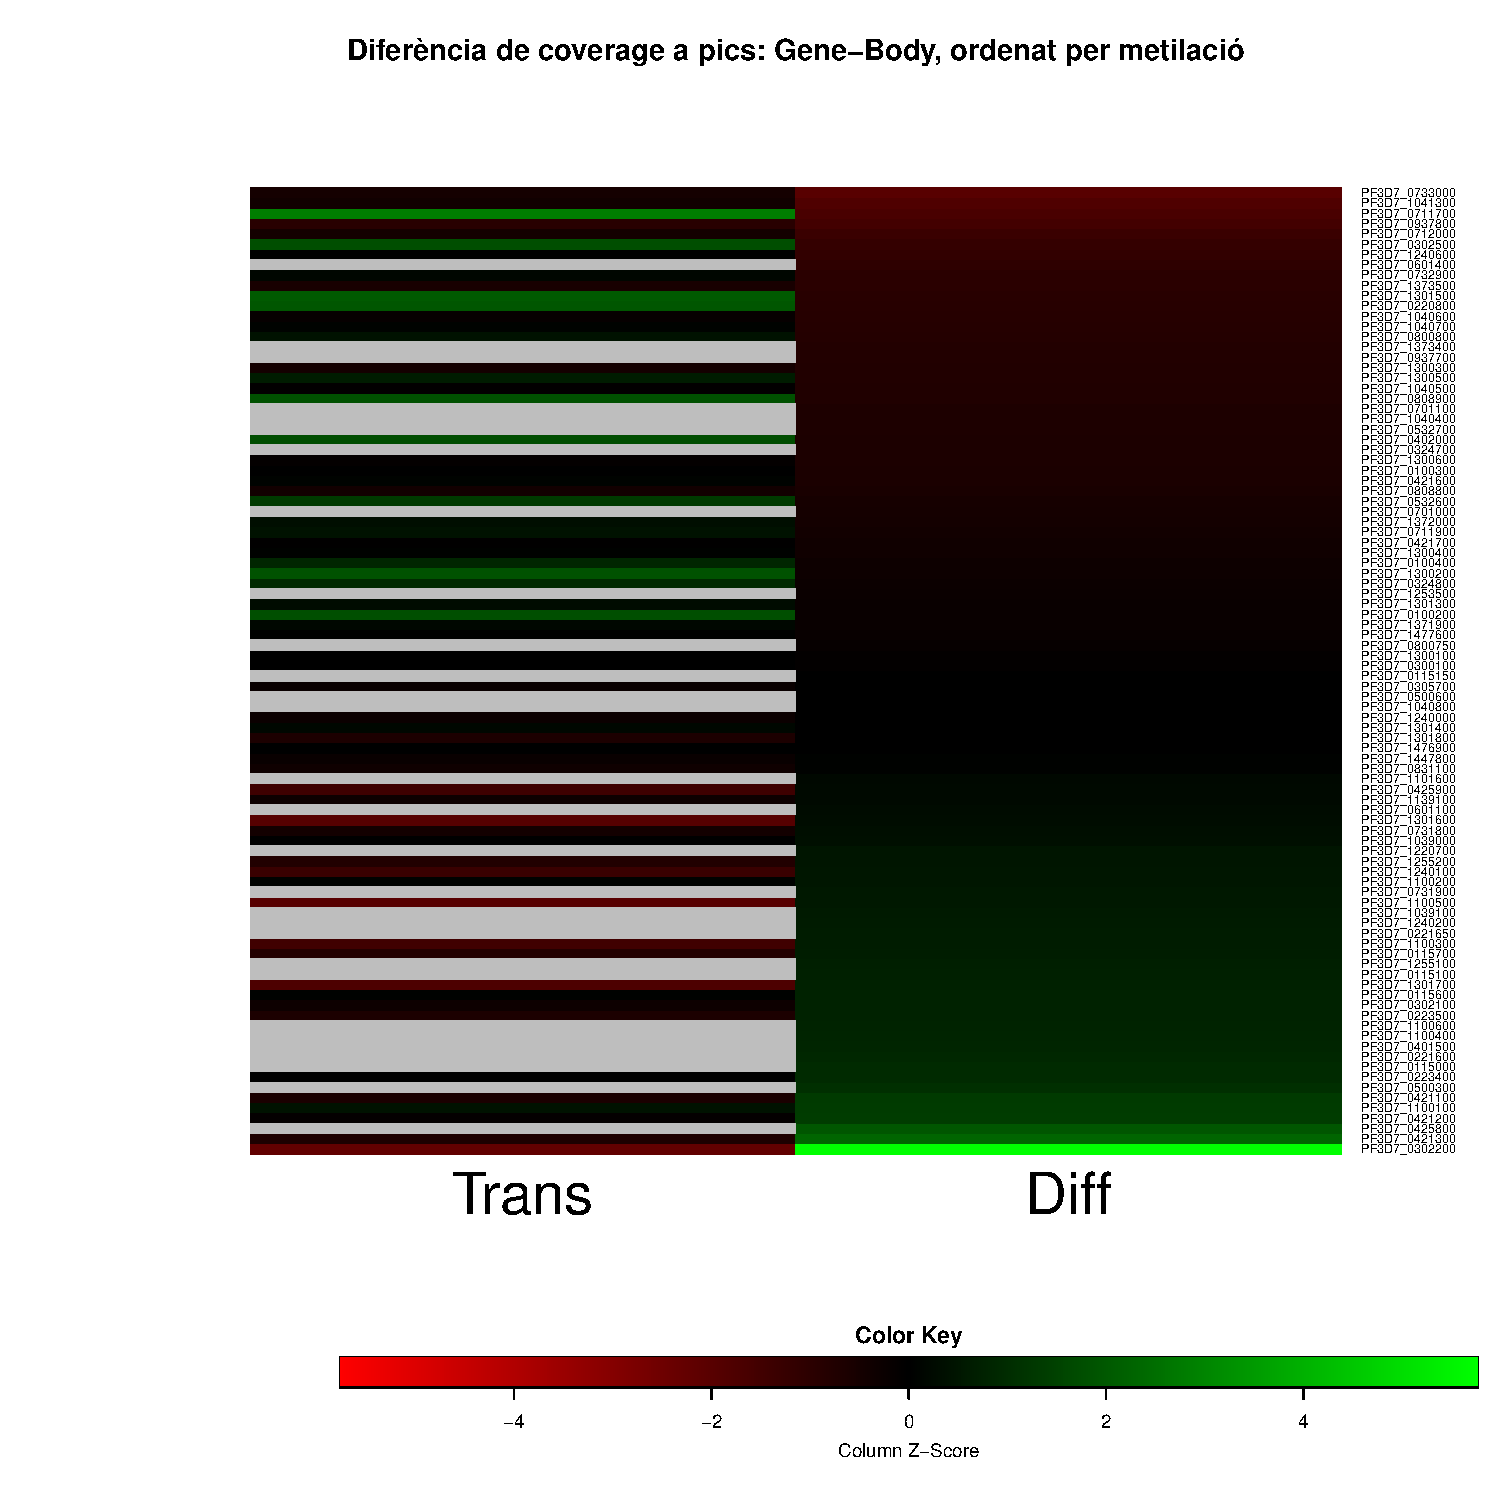
\includegraphics[width=.9\linewidth]{figure/minimal-heat_difpeak_cov_dif_metord-1} 

}



\end{knitrout}
% -----------------------------------------------------------------------------------------------------------------------------------------
% ---------------------------------------------------------  RESTA DE GRÀFICS -------------------------------------------------------------
\clearpage
\section{Resta de gràfics}
\section{Percentatge de metilació}
\subsection{Gene-body}
\begin{knitrout}
\definecolor{shadecolor}{rgb}{0.969, 0.969, 0.969}\color{fgcolor}

{\centering 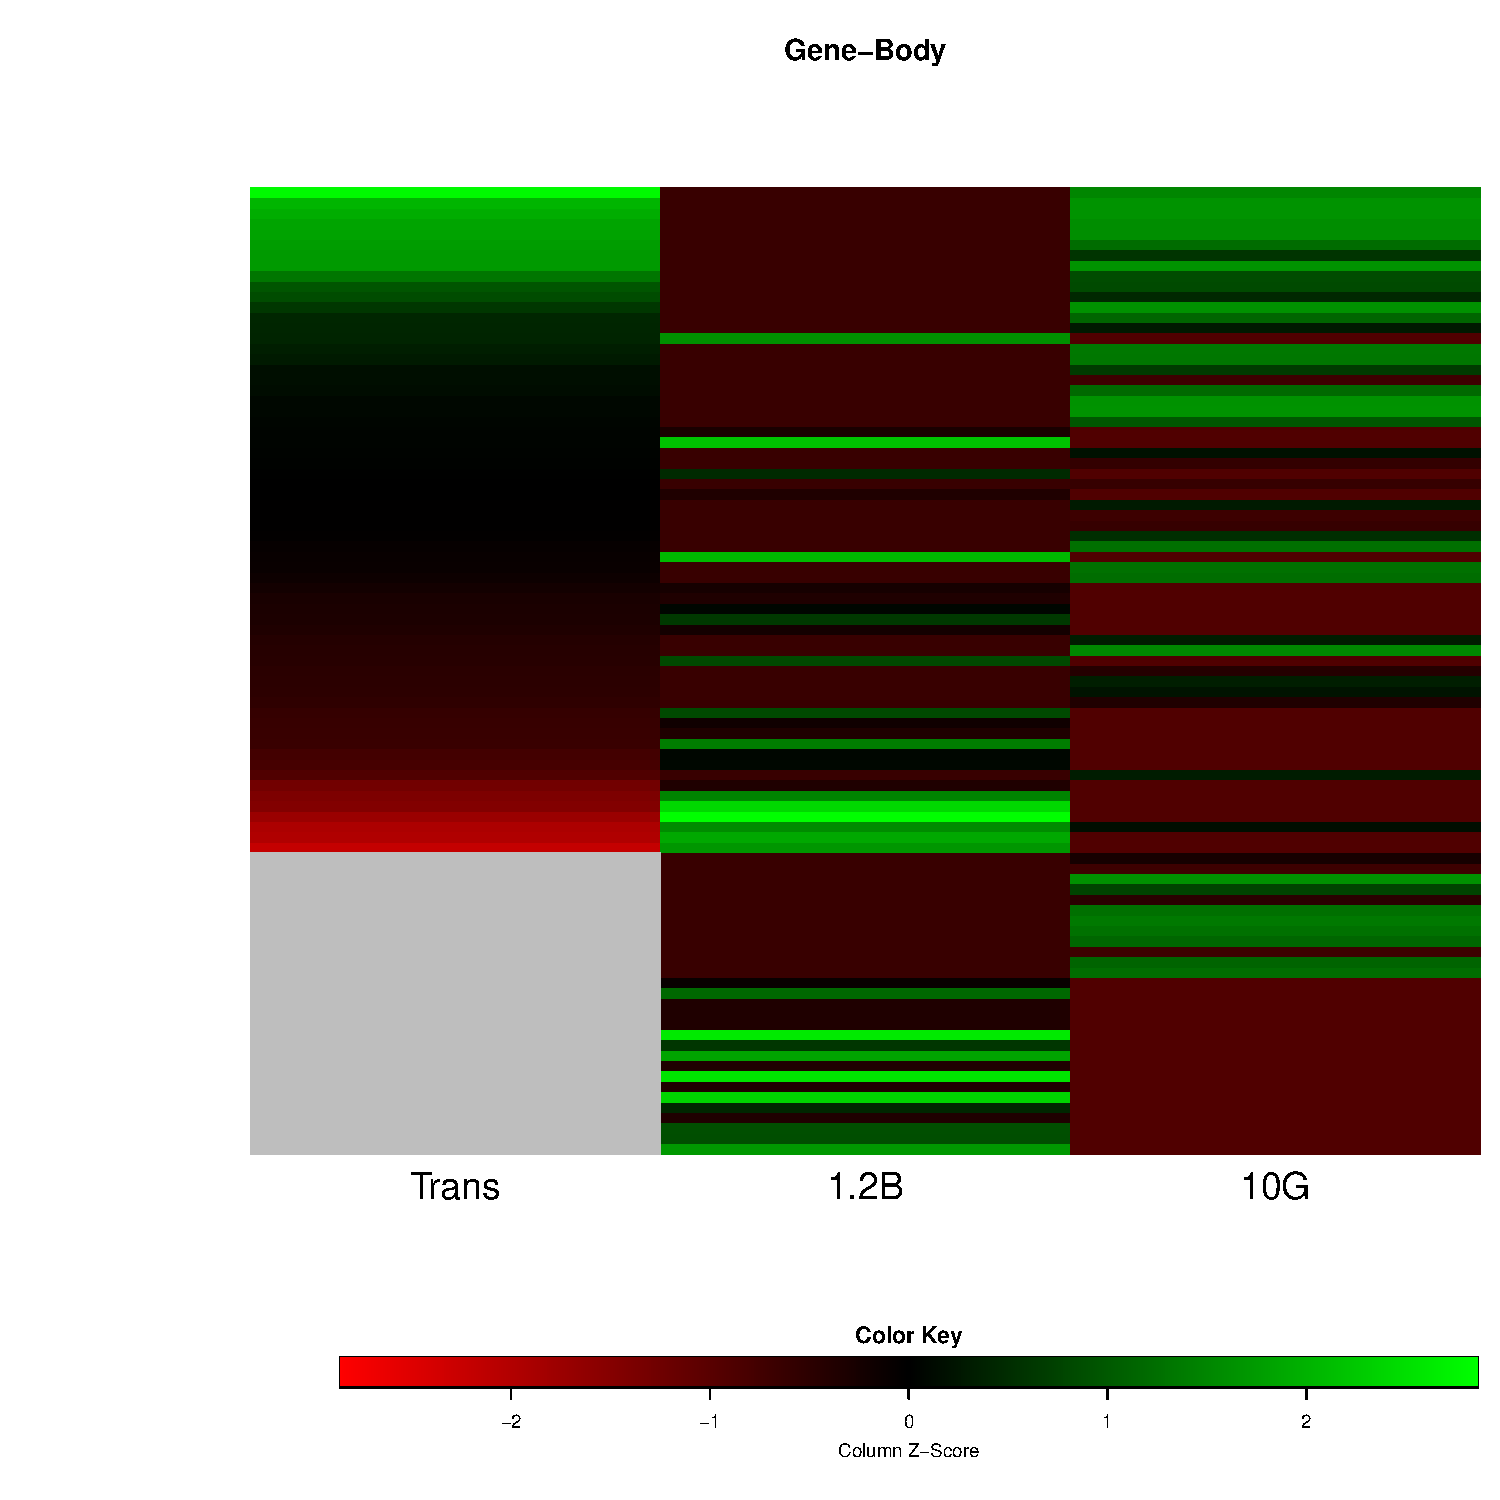
\includegraphics[width=.9\linewidth]{figure/minimal-heatmap_gene-1} 

}



\end{knitrout}
\clearpage
\subsection{TSS}
En aquest gràfic en comptes d'ordenar els gens en funció de la primera columna s'han ordenat "sols" seguint l'algoritme de clustering de la funció "heatmap" de R.
\begin{knitrout}
\definecolor{shadecolor}{rgb}{0.969, 0.969, 0.969}\color{fgcolor}

{\centering 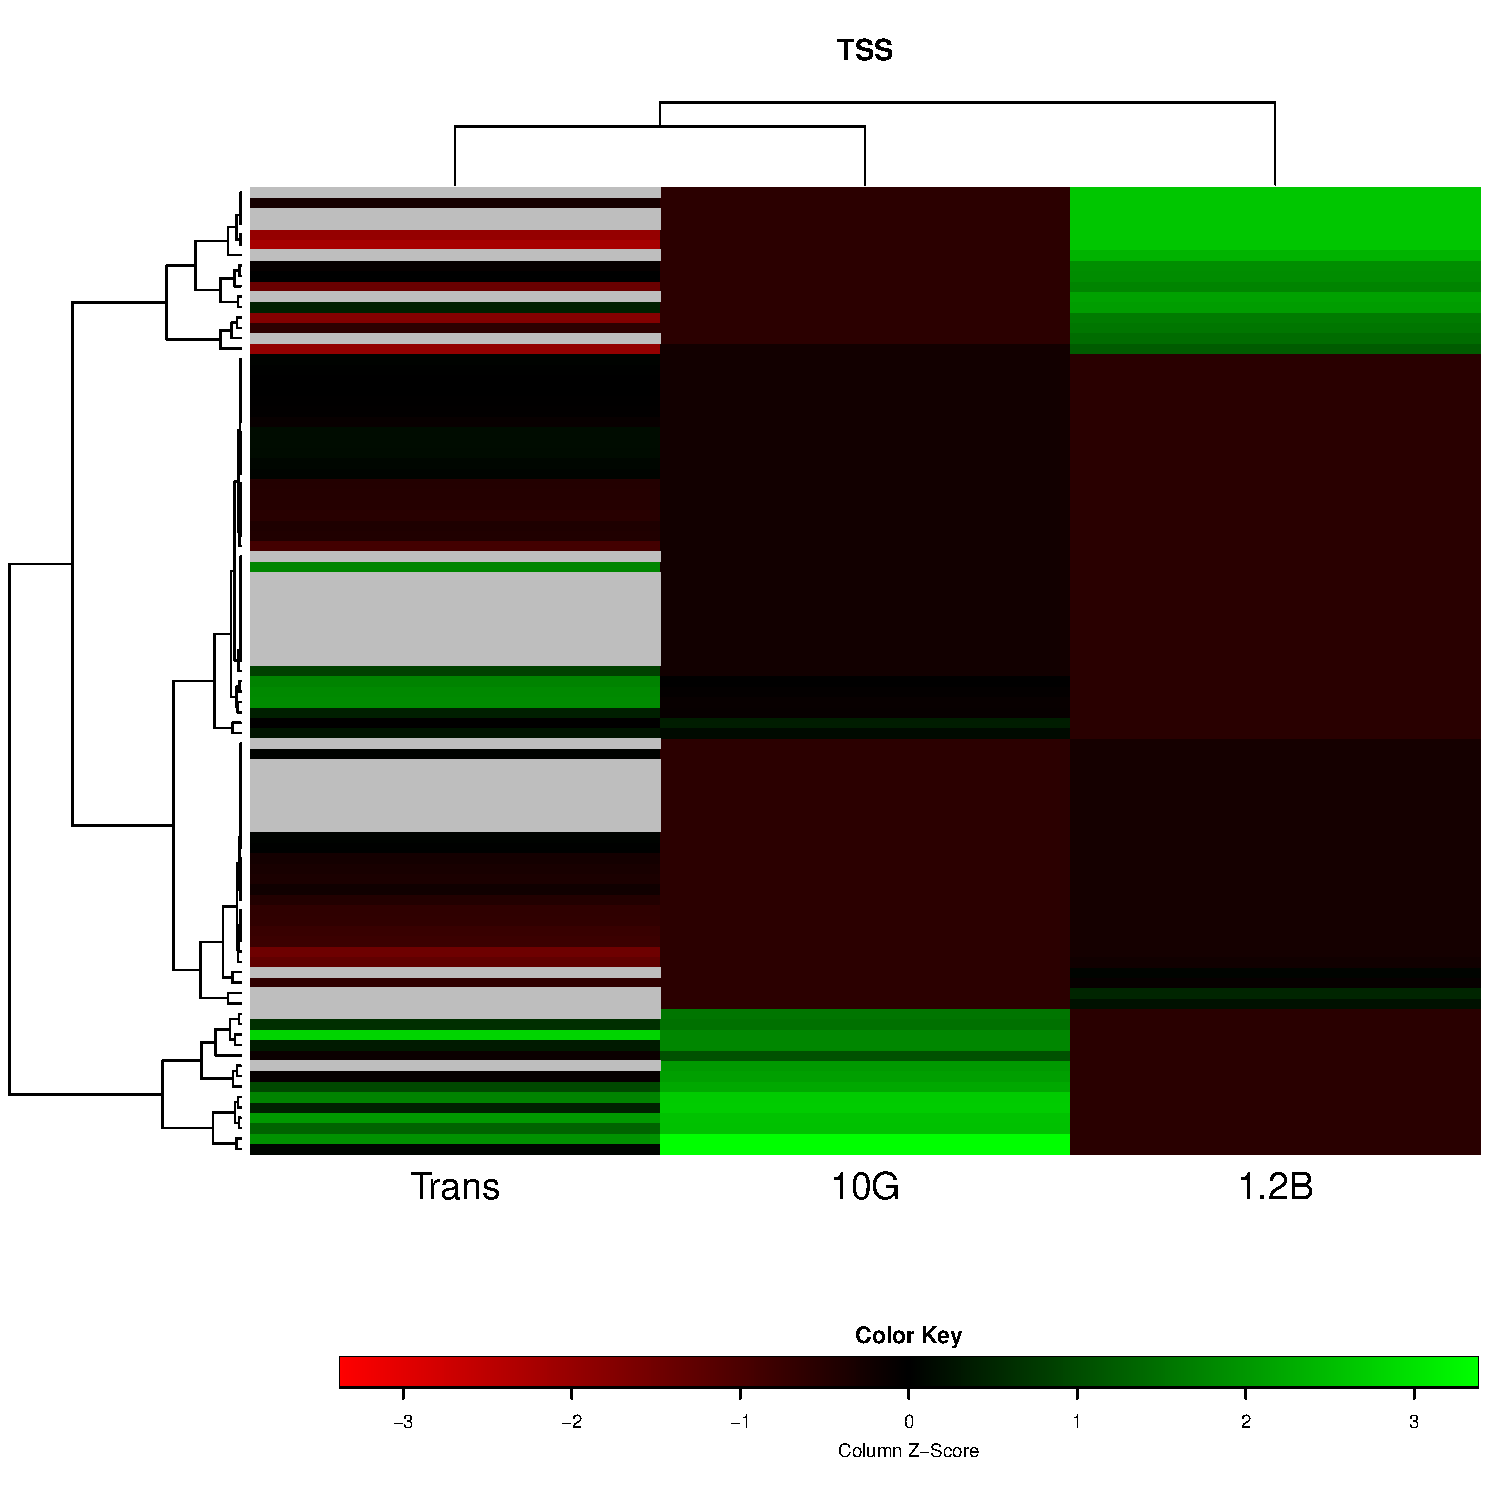
\includegraphics[width=.9\linewidth]{figure/minimal-heatmap_tss-1} 

}



\end{knitrout}
\clearpage
\subsection{Gene + TSS}
\begin{knitrout}
\definecolor{shadecolor}{rgb}{0.969, 0.969, 0.969}\color{fgcolor}

{\centering 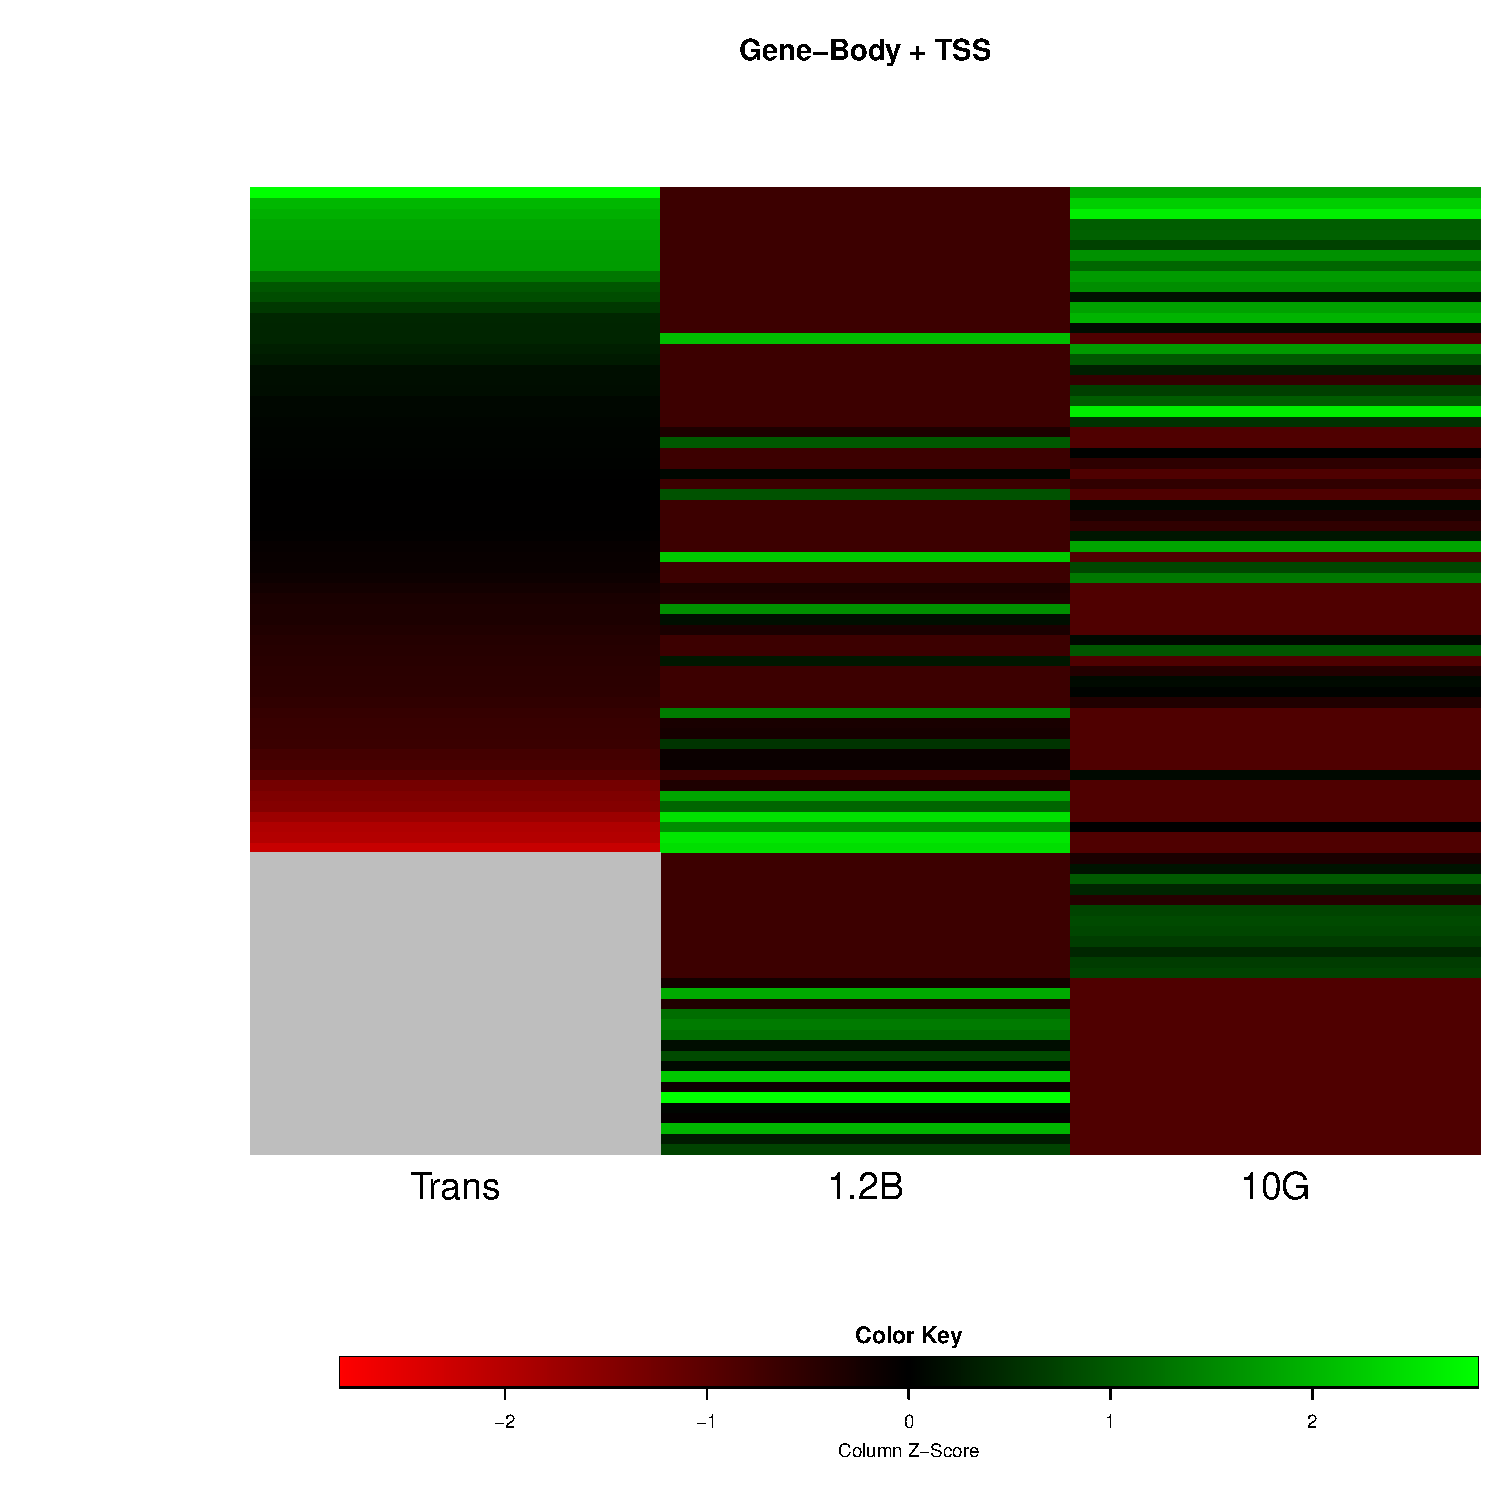
\includegraphics[width=.9\linewidth]{figure/minimal-heatmap_gene_tss-1} 

}



\end{knitrout}
\clearpage
\subsection{TTS}
\begin{knitrout}
\definecolor{shadecolor}{rgb}{0.969, 0.969, 0.969}\color{fgcolor}

{\centering 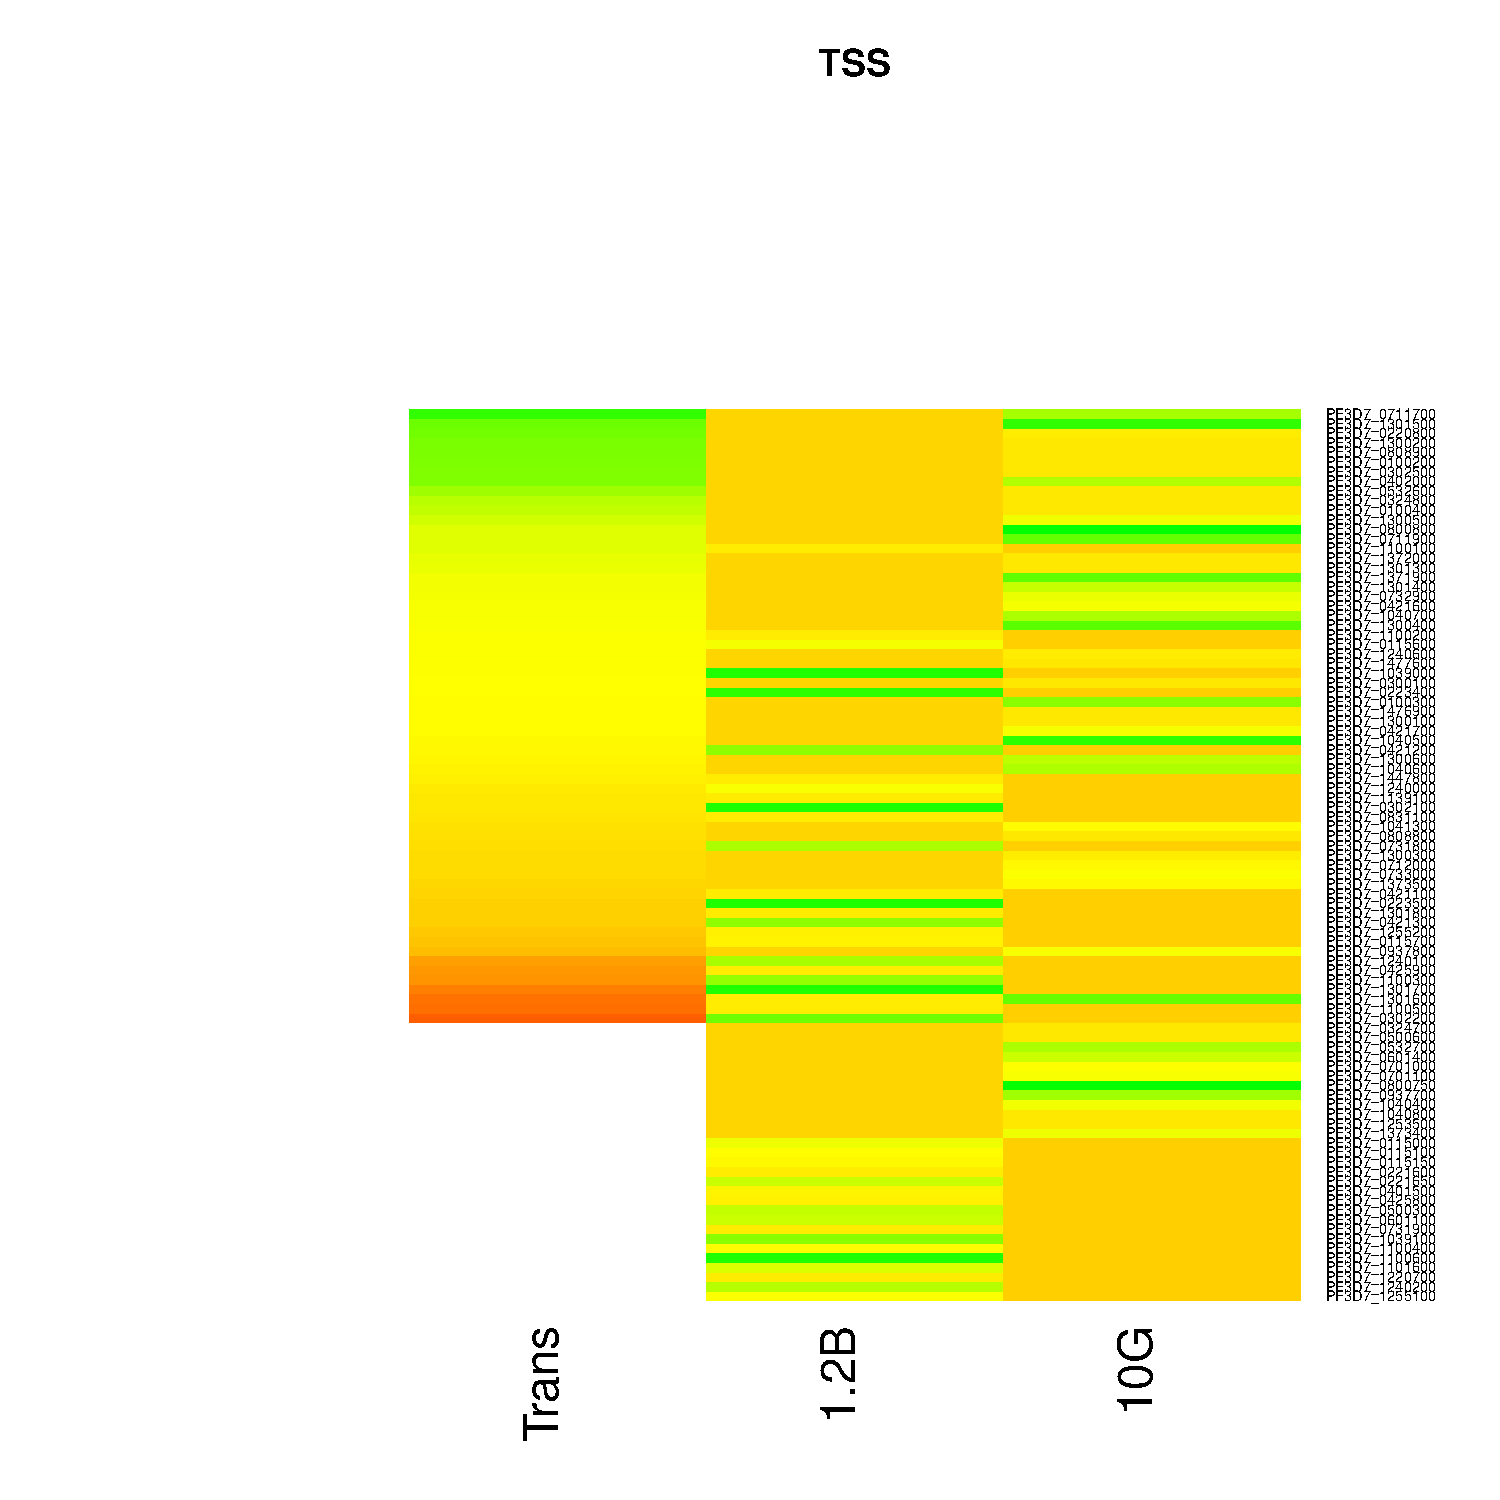
\includegraphics[width=.9\linewidth]{figure/minimal-heatmap_tts-1} 

}



\end{knitrout}

\clearpage
\section{Coverage}
\subsection{Coverage Gene Body}
\begin{knitrout}
\definecolor{shadecolor}{rgb}{0.969, 0.969, 0.969}\color{fgcolor}

{\centering 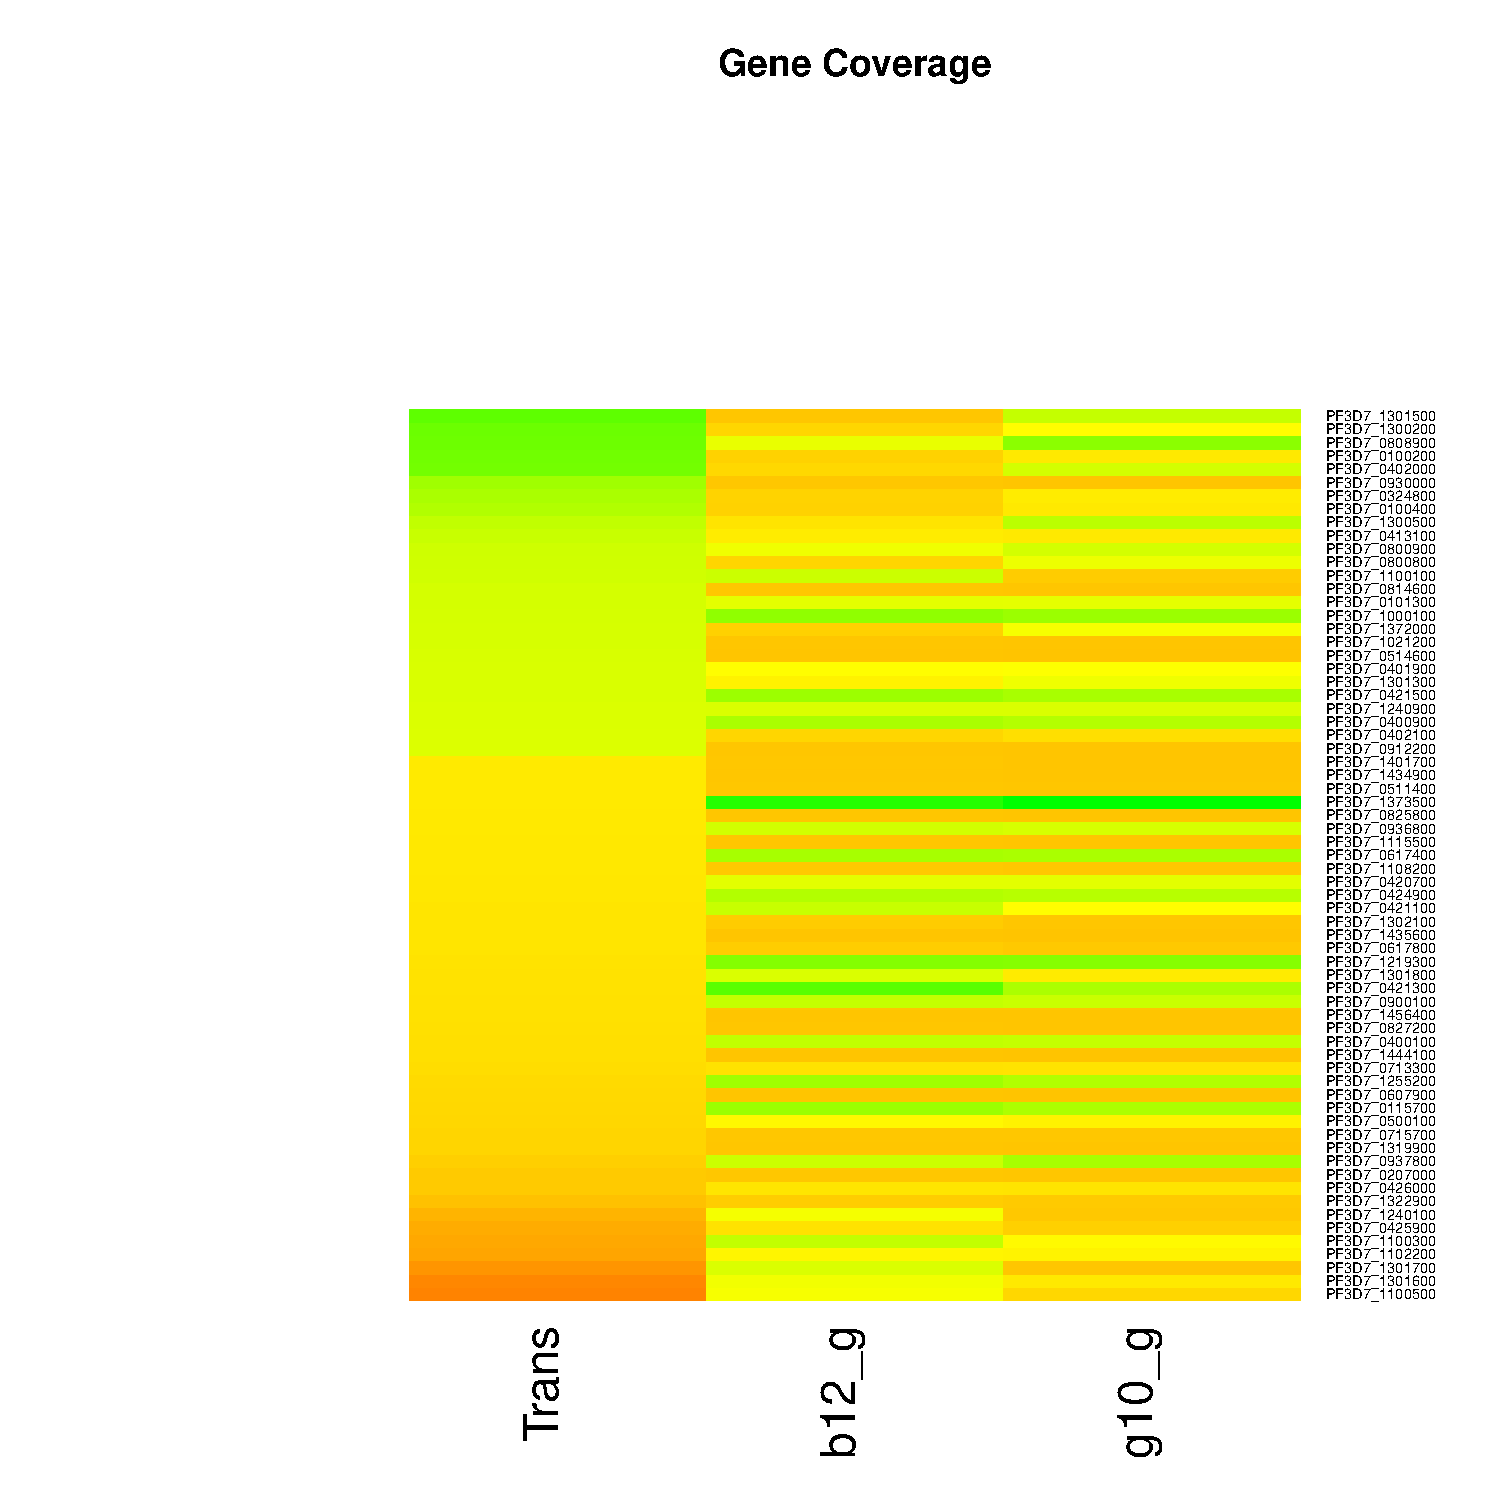
\includegraphics[width=.9\linewidth]{figure/minimal-heat_cov_gene-1} 

}



\end{knitrout}
\clearpage
\subsection{Coverage 5'}
\begin{knitrout}
\definecolor{shadecolor}{rgb}{0.969, 0.969, 0.969}\color{fgcolor}

{\centering 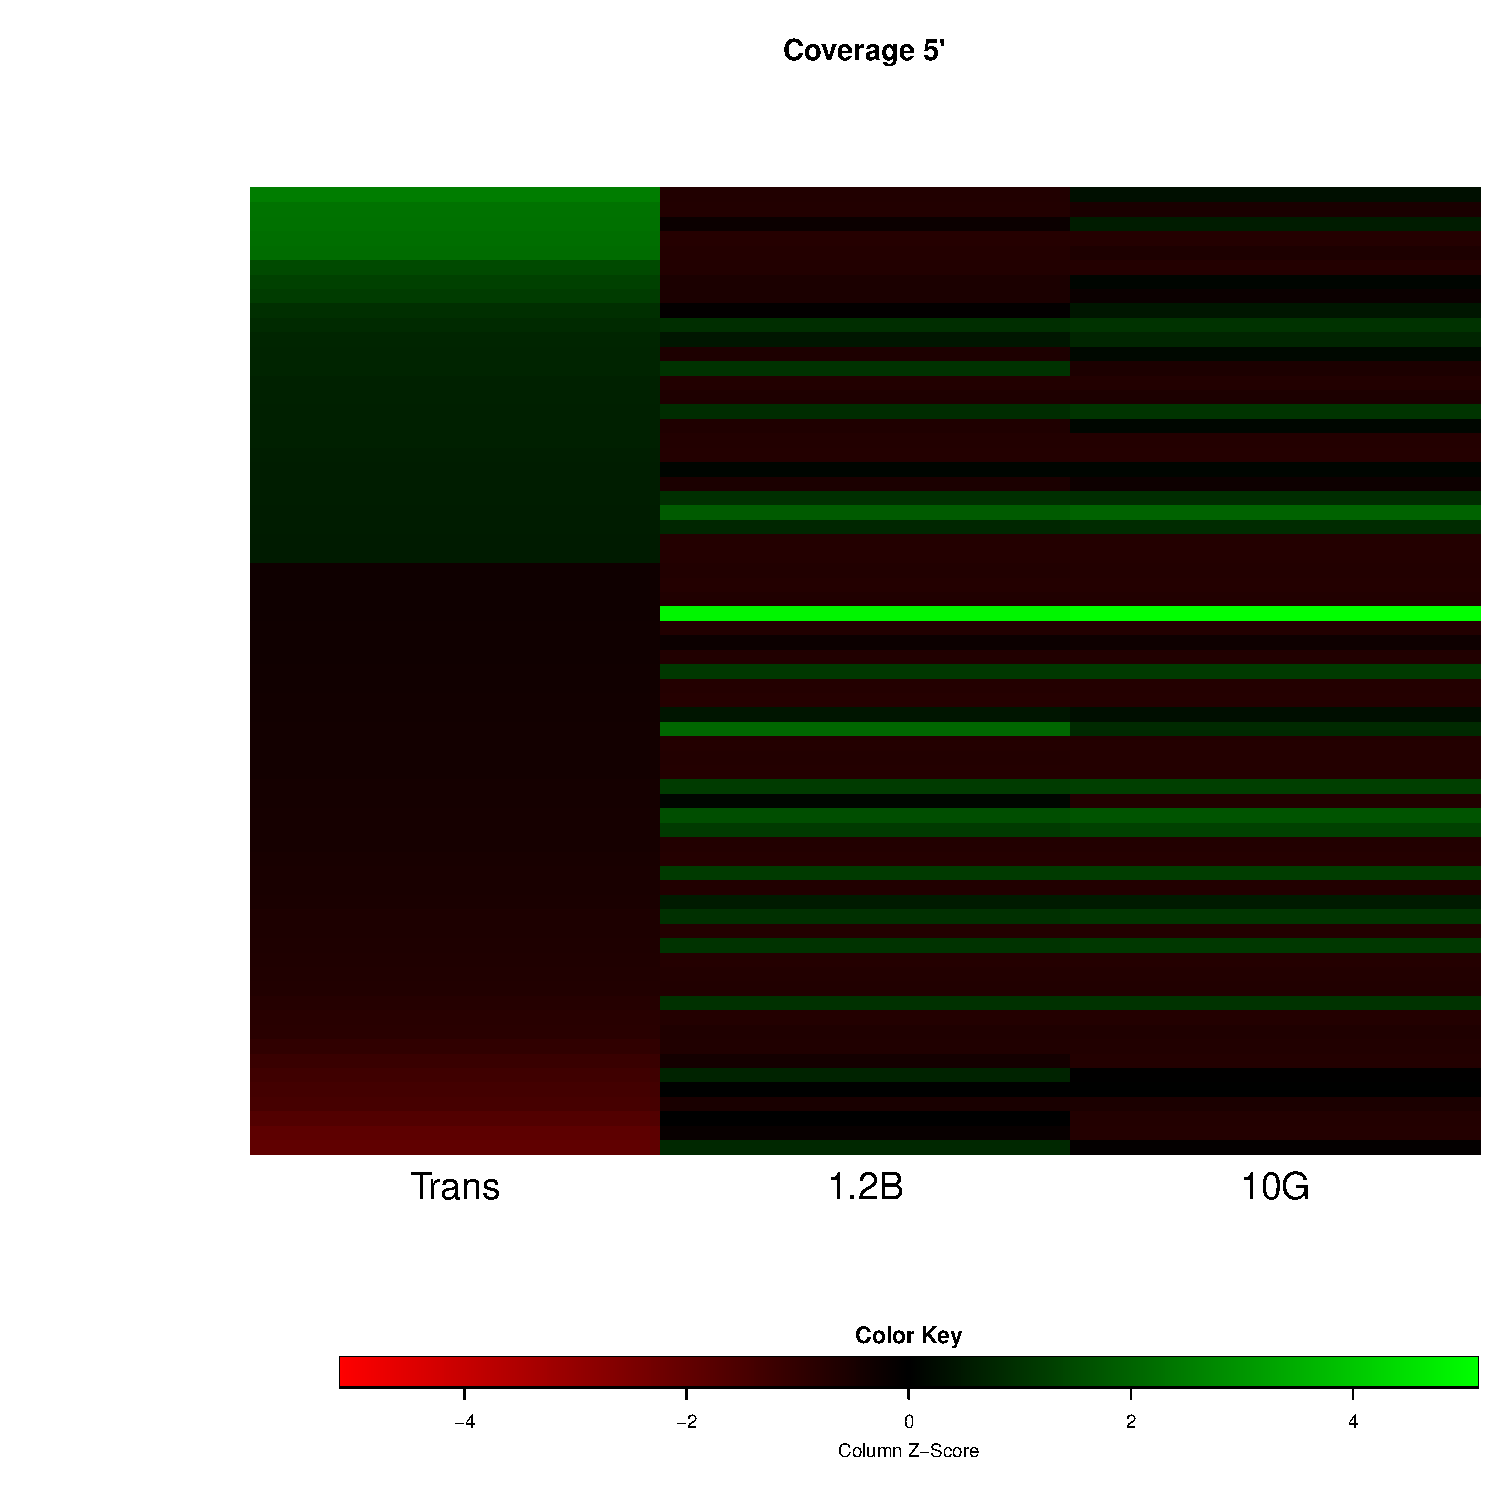
\includegraphics[width=.9\linewidth]{figure/minimal-heat_cov_tss-1} 

}



\end{knitrout}
\clearpage
\clearpage
\subsection{Coverage 3'}
\begin{knitrout}
\definecolor{shadecolor}{rgb}{0.969, 0.969, 0.969}\color{fgcolor}

{\centering 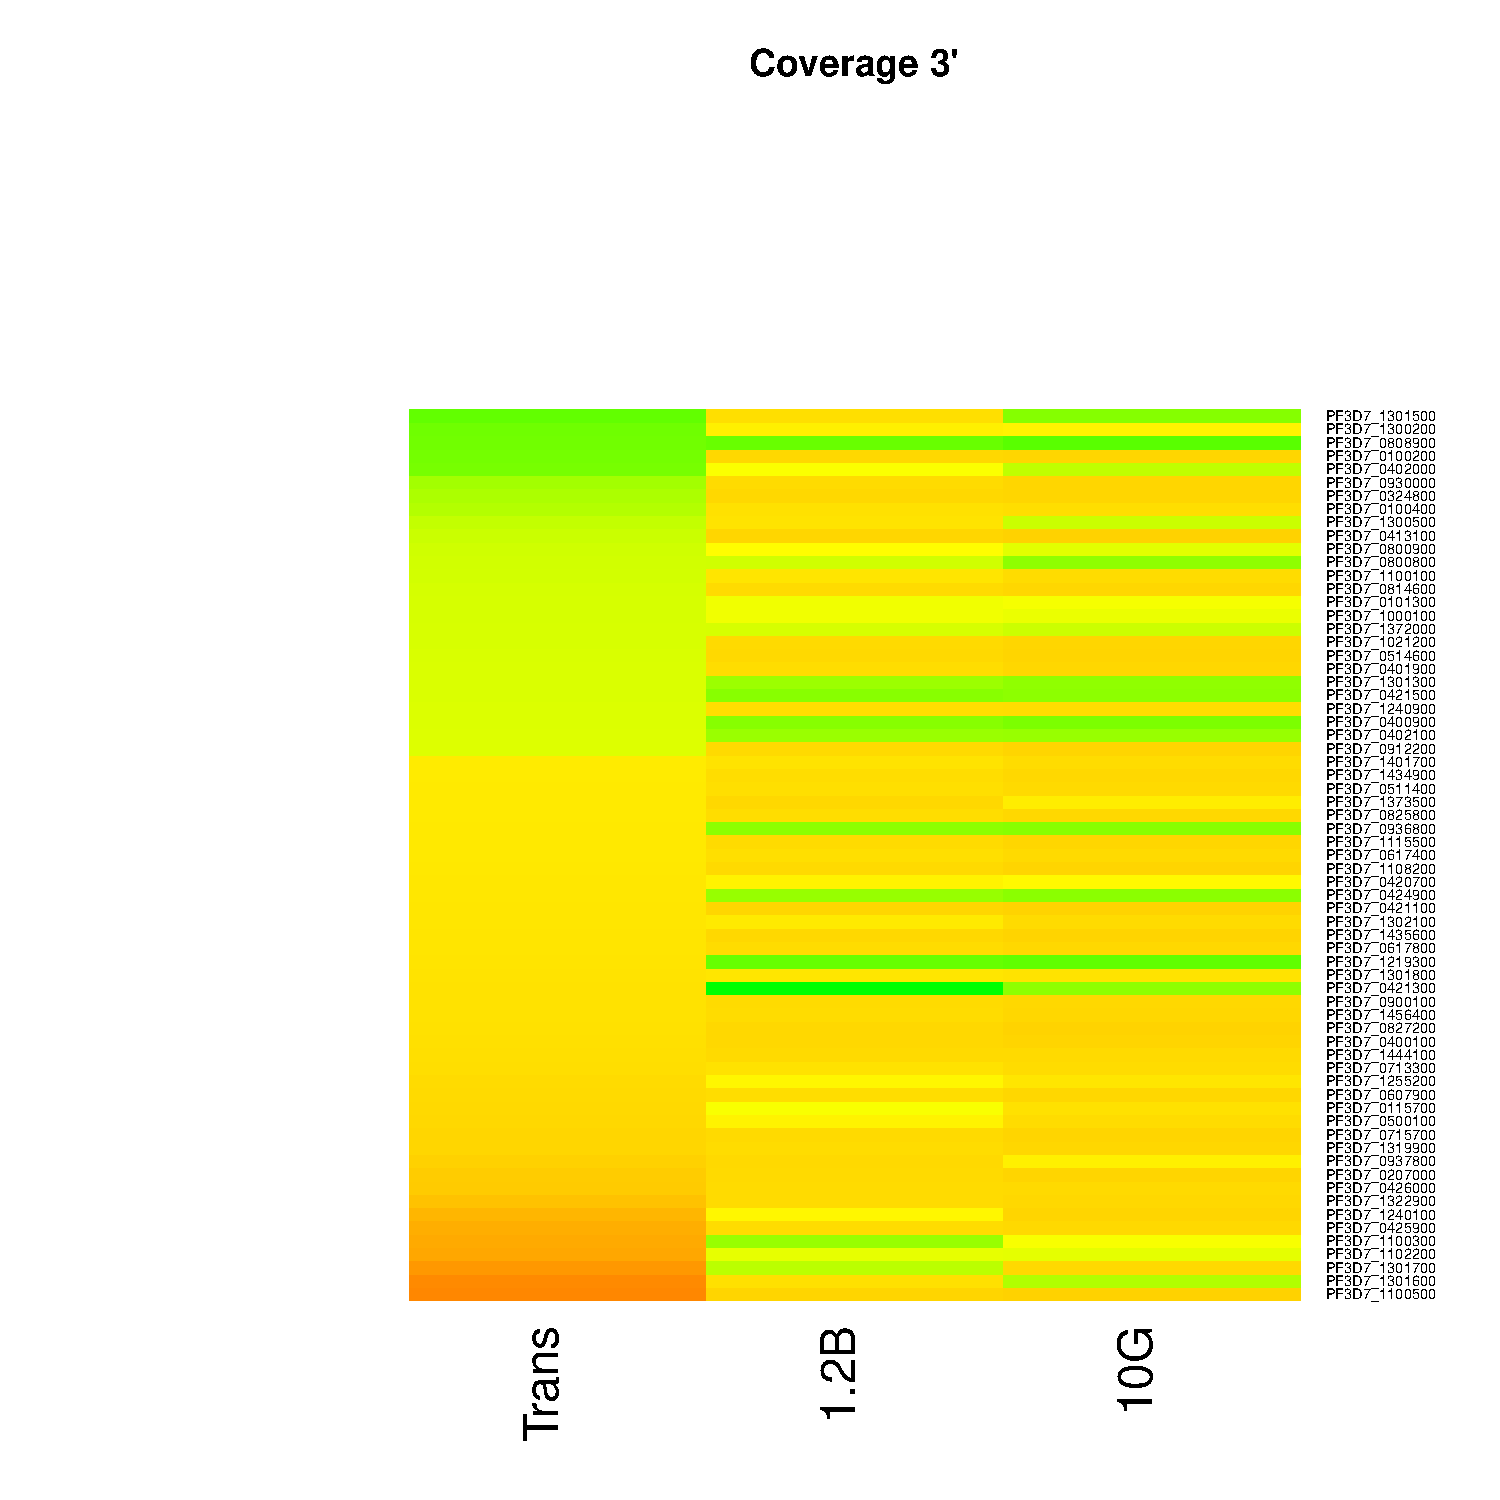
\includegraphics[width=.9\linewidth]{figure/minimal-heat_cov_tts-1} 

}



\end{knitrout}
\clearpage

\section{Diferència de coverage}
\subsection{Diferència de Coverage a 5', filtrat per diferència de transcripció}
\begin{knitrout}
\definecolor{shadecolor}{rgb}{0.969, 0.969, 0.969}\color{fgcolor}

{\centering 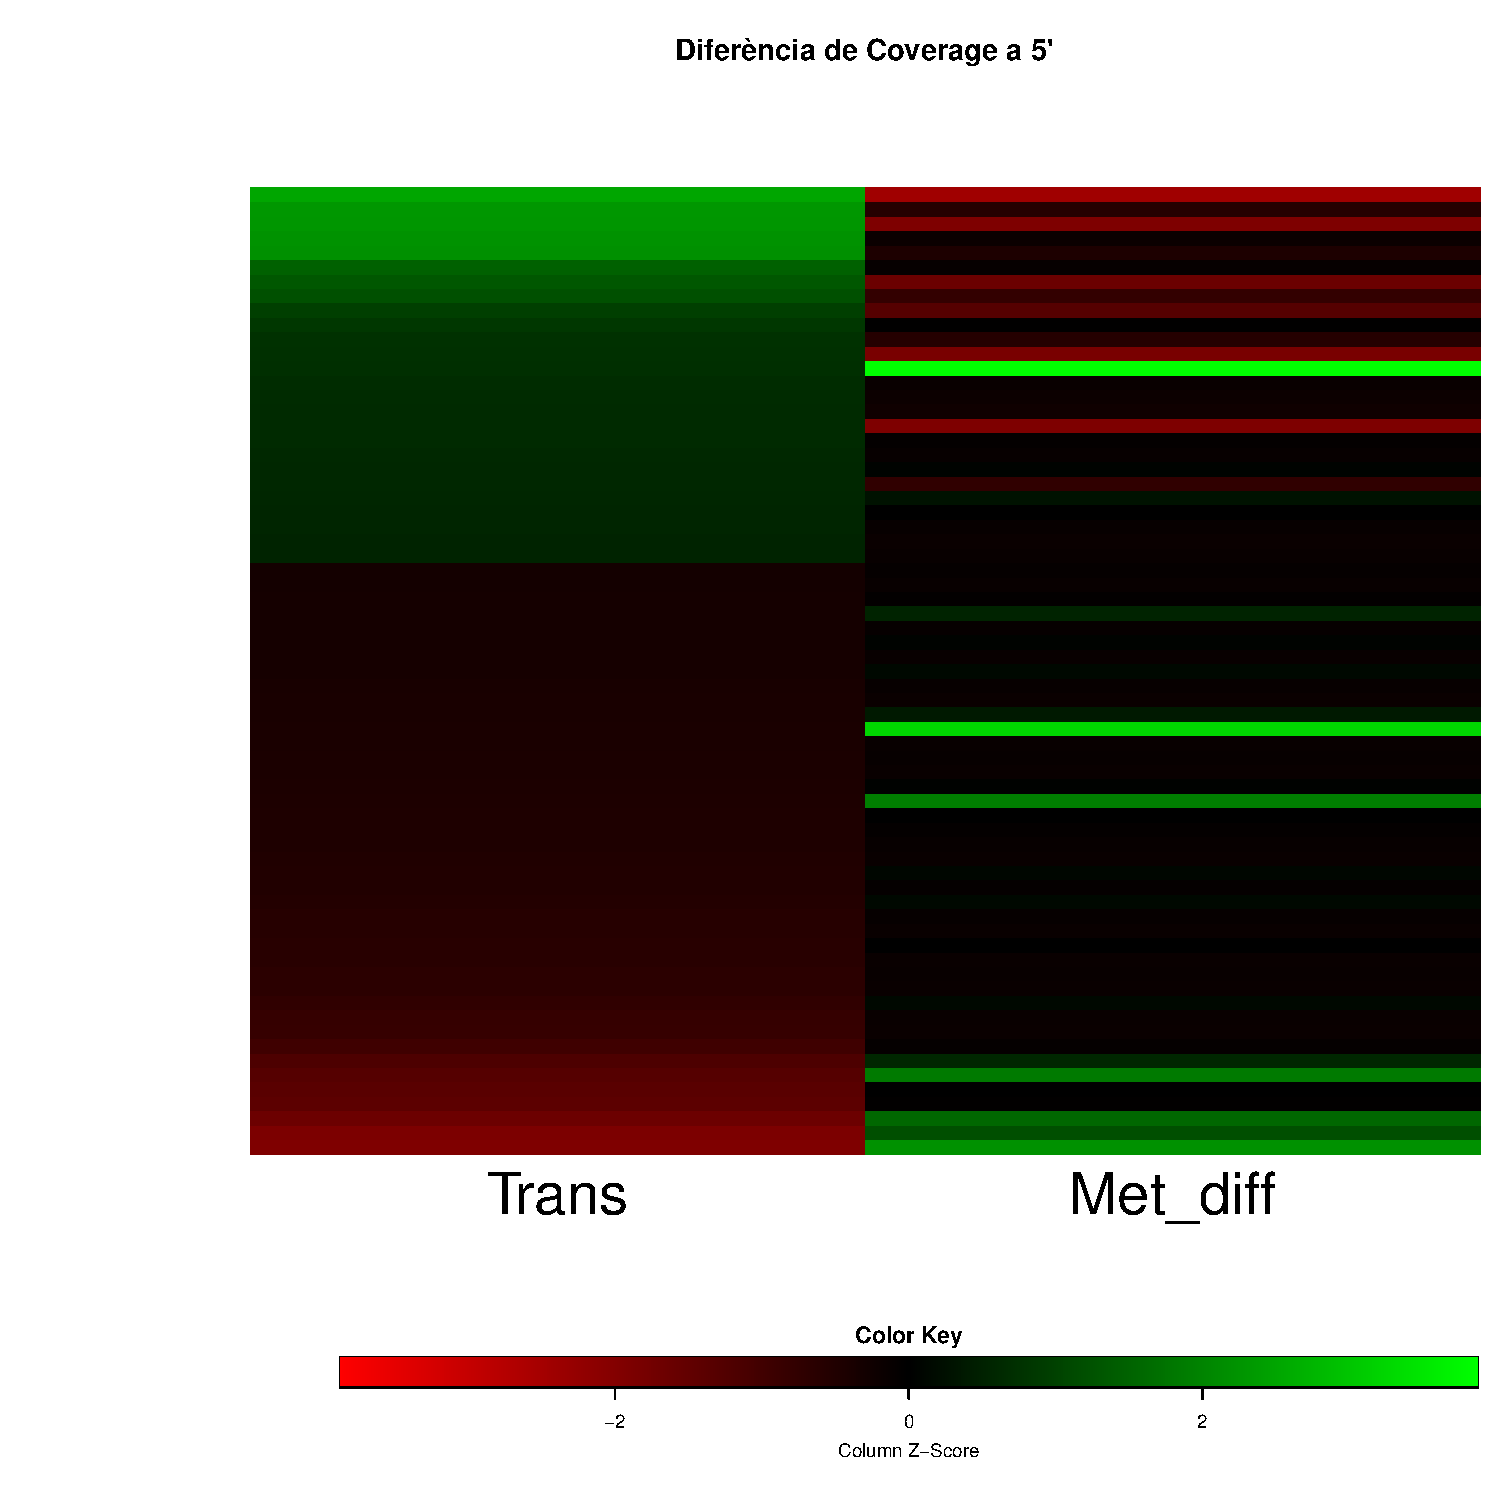
\includegraphics[width=.9\linewidth]{figure/minimal-_heat_cov_diff_5-1} 

}



\end{knitrout}
\clearpage
\subsection{Diferència de Coverage a genebody, filtrat per diferència de transcripció}
\begin{knitrout}
\definecolor{shadecolor}{rgb}{0.969, 0.969, 0.969}\color{fgcolor}

{\centering 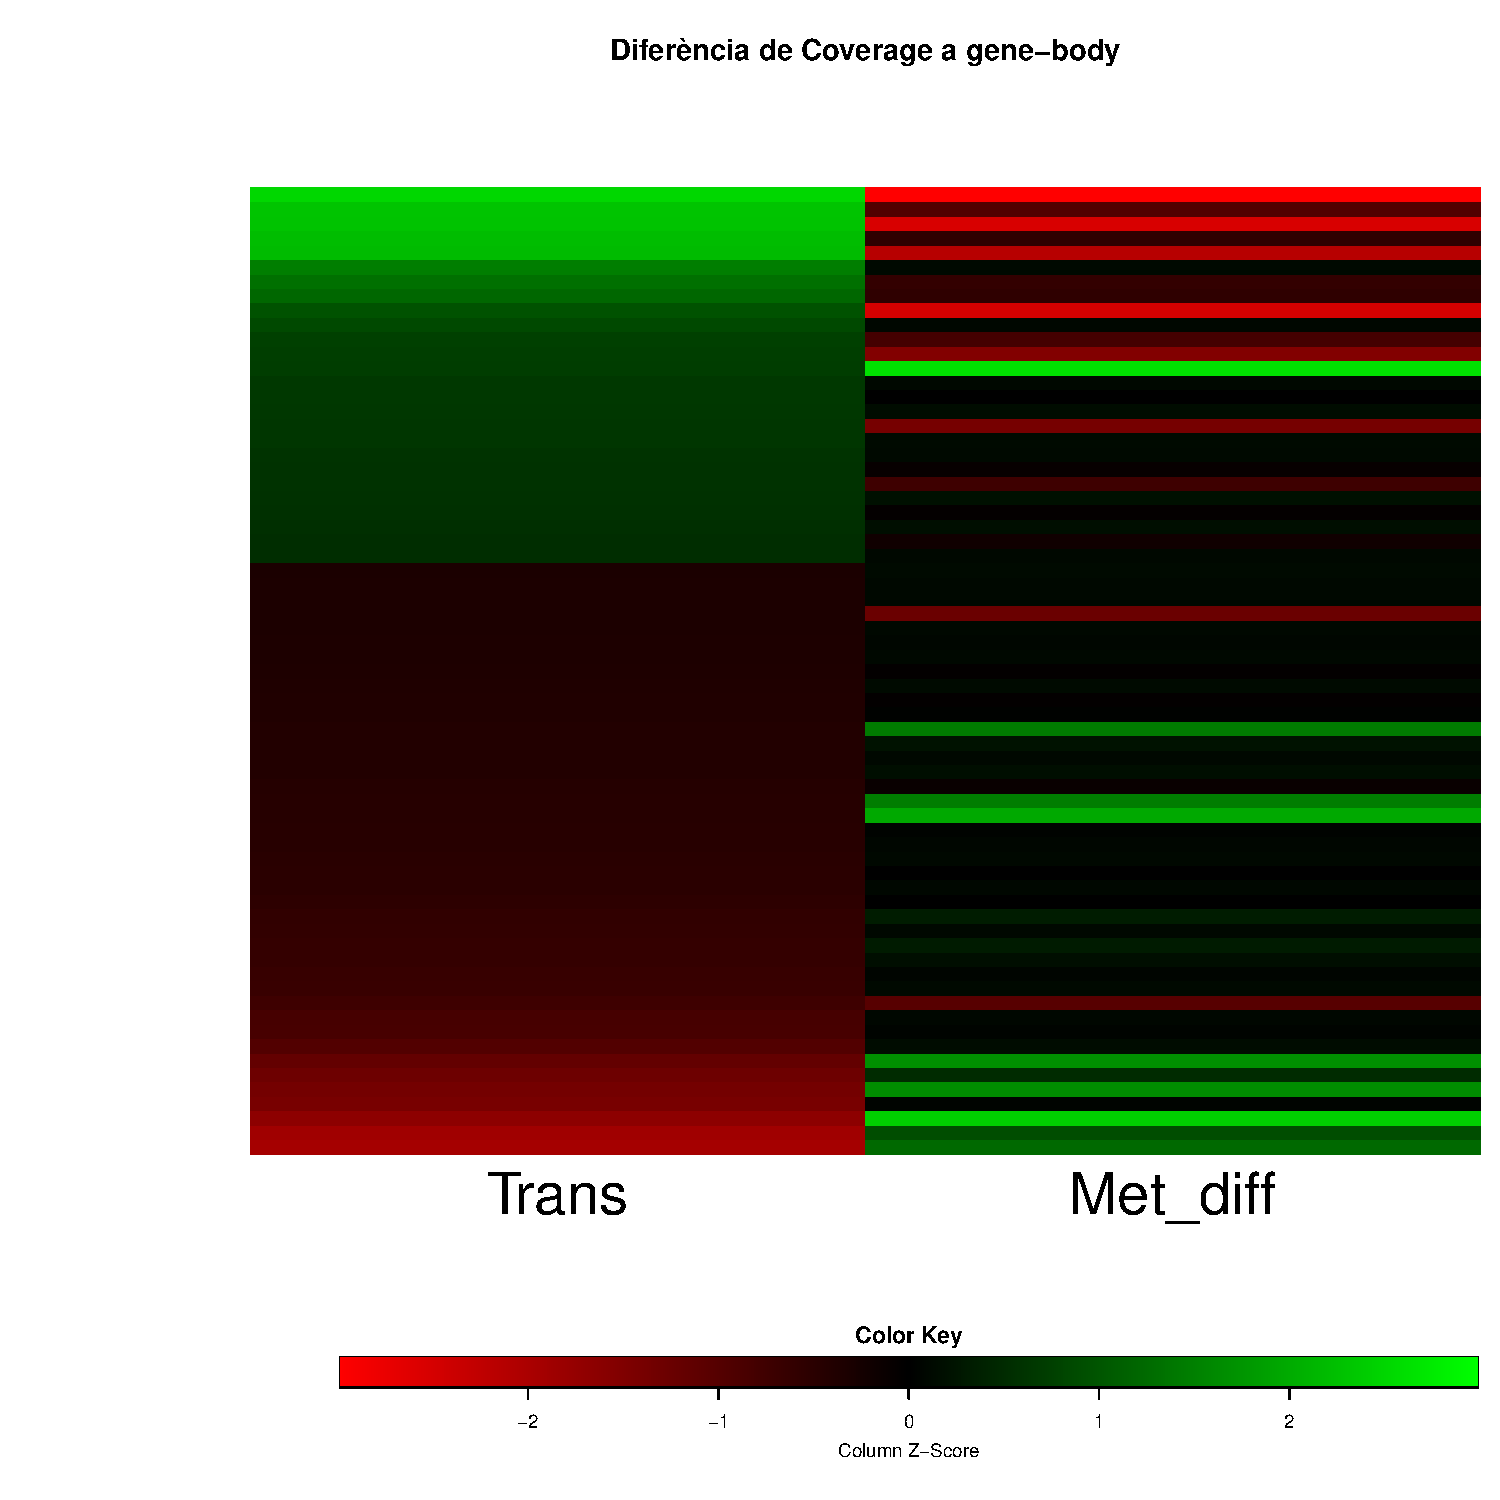
\includegraphics[width=.9\linewidth]{figure/minimal-_heat_cov_diff_body-1} 

}



\end{knitrout}
\clearpage
\subsection{Diferència de Coverage 5'genebody, filtrat per diferència de transcripció}
\begin{knitrout}
\definecolor{shadecolor}{rgb}{0.969, 0.969, 0.969}\color{fgcolor}

{\centering 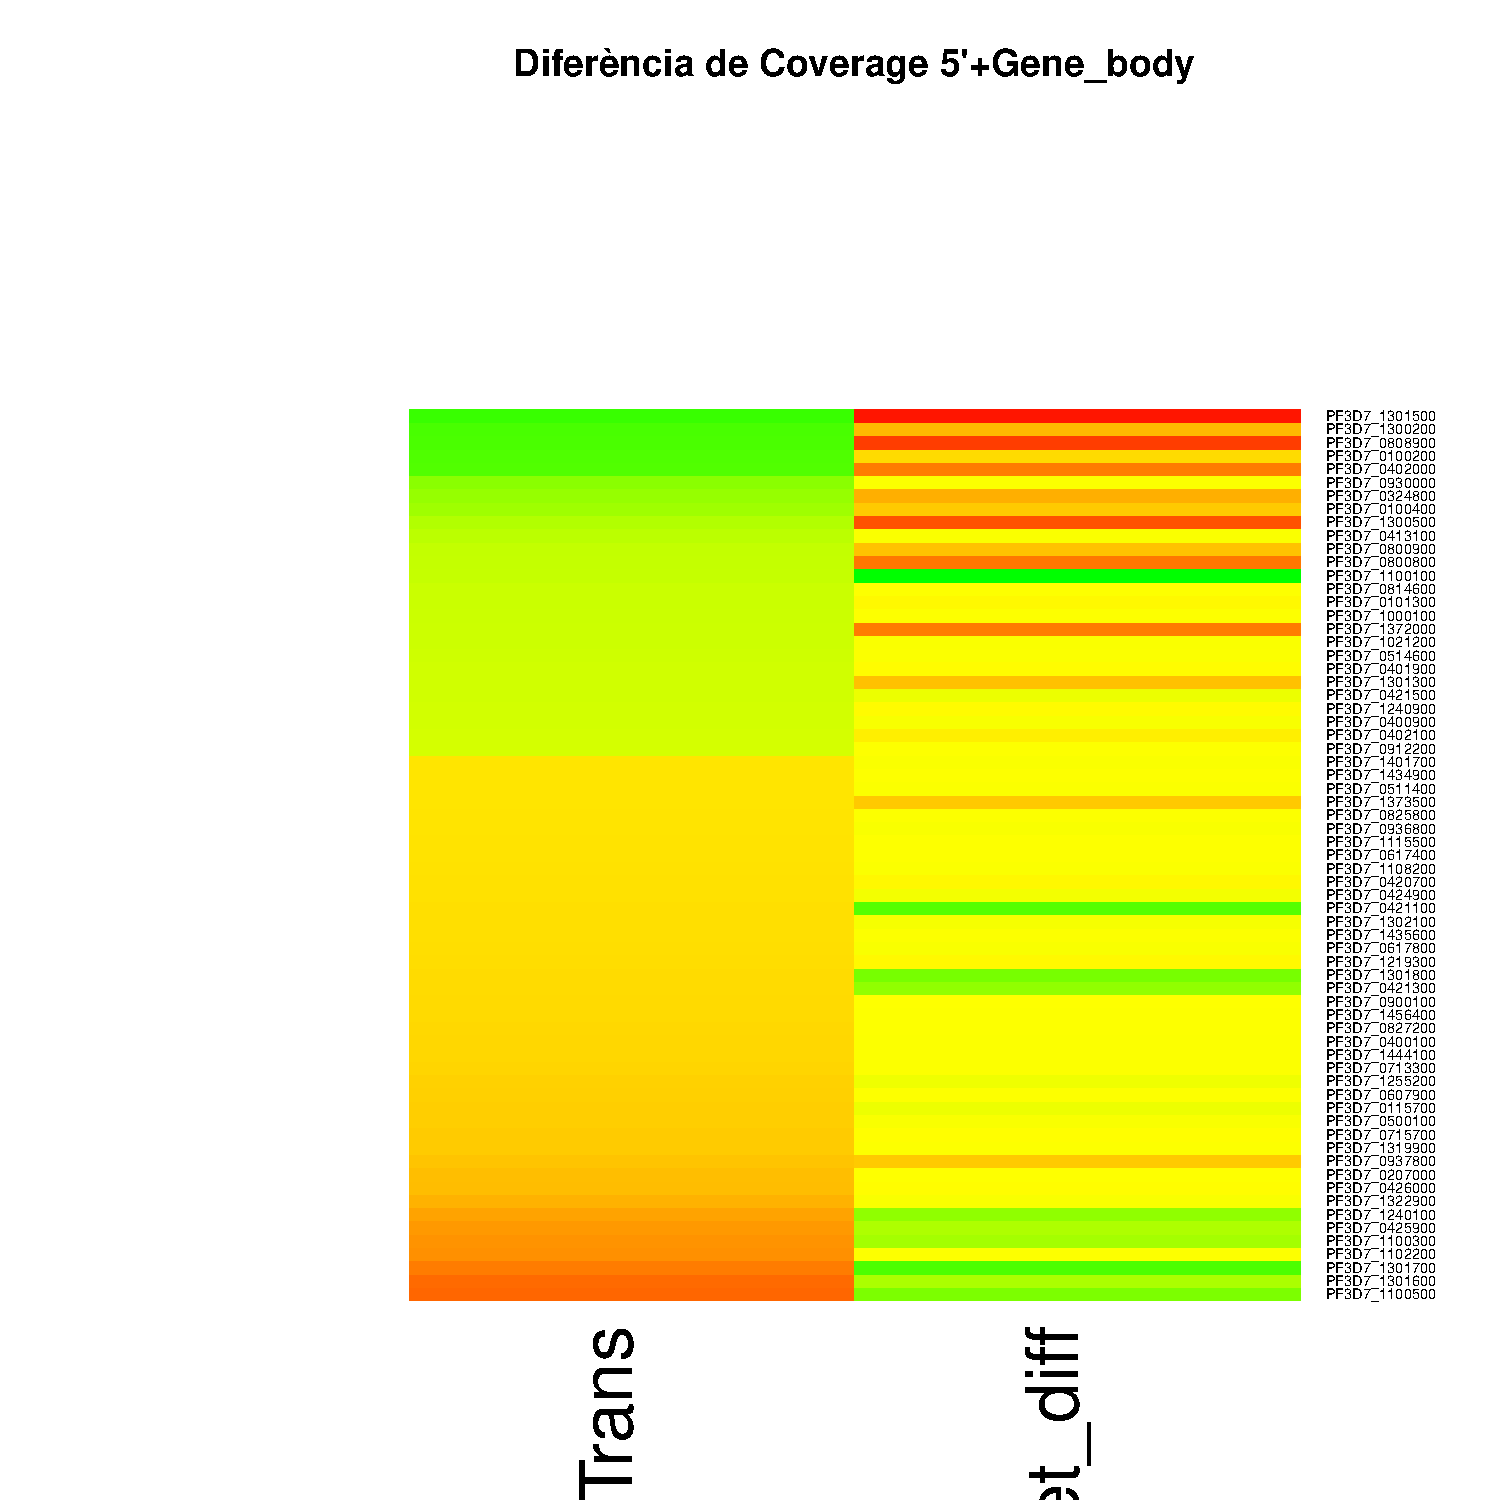
\includegraphics[width=.9\linewidth]{figure/minimal-_heat_cov_diff_body5-1} 

}



\end{knitrout}
\clearpage
\subsection{Diferència de Coverage a 3', filtrat per diferència de transcripció}
\begin{knitrout}
\definecolor{shadecolor}{rgb}{0.969, 0.969, 0.969}\color{fgcolor}

{\centering 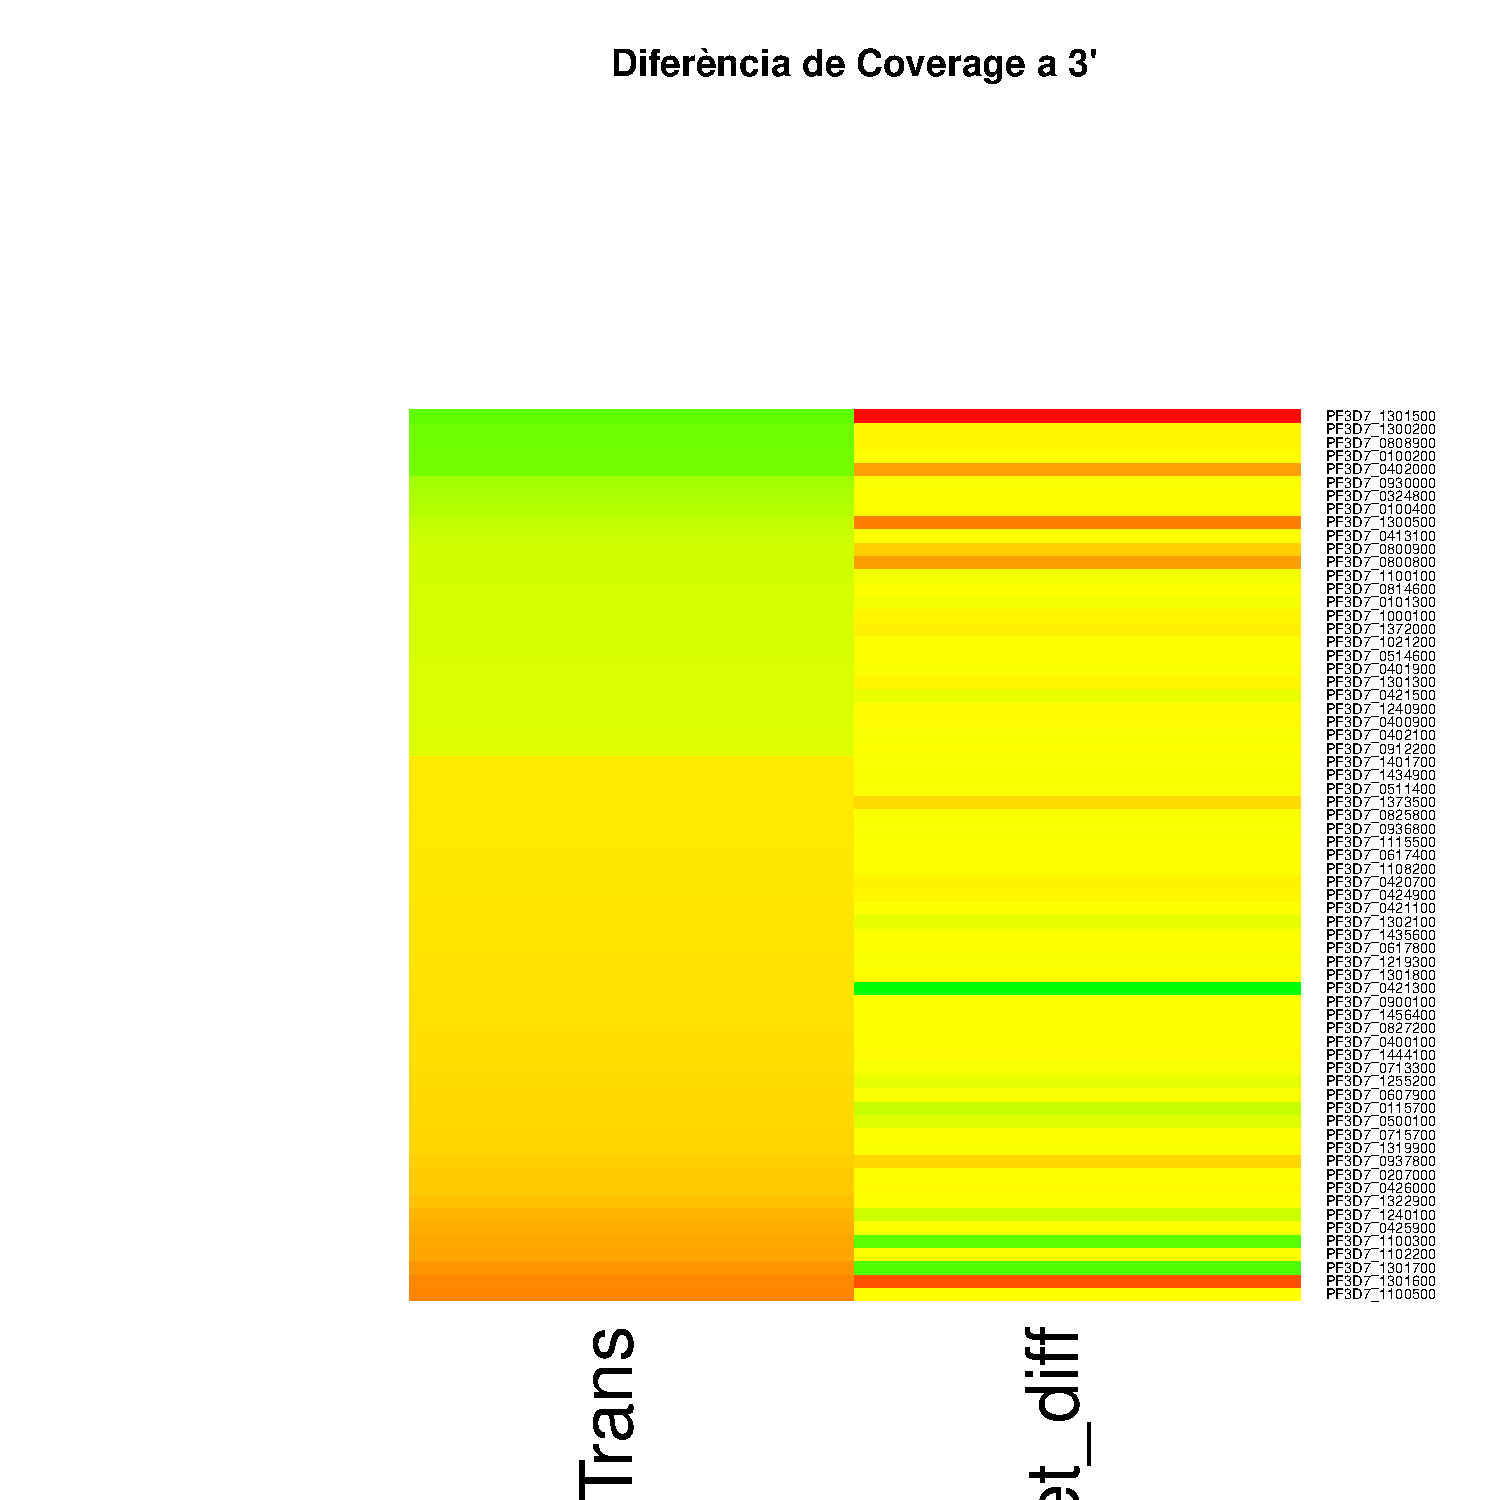
\includegraphics[width=.9\linewidth]{figure/minimal-_heat_cov_diff_3-1} 

}



\end{knitrout}



\clearpage
\section{Multiple-regression Model}
\begin{knitrout}
\definecolor{shadecolor}{rgb}{0.969, 0.969, 0.969}\color{fgcolor}

{\centering 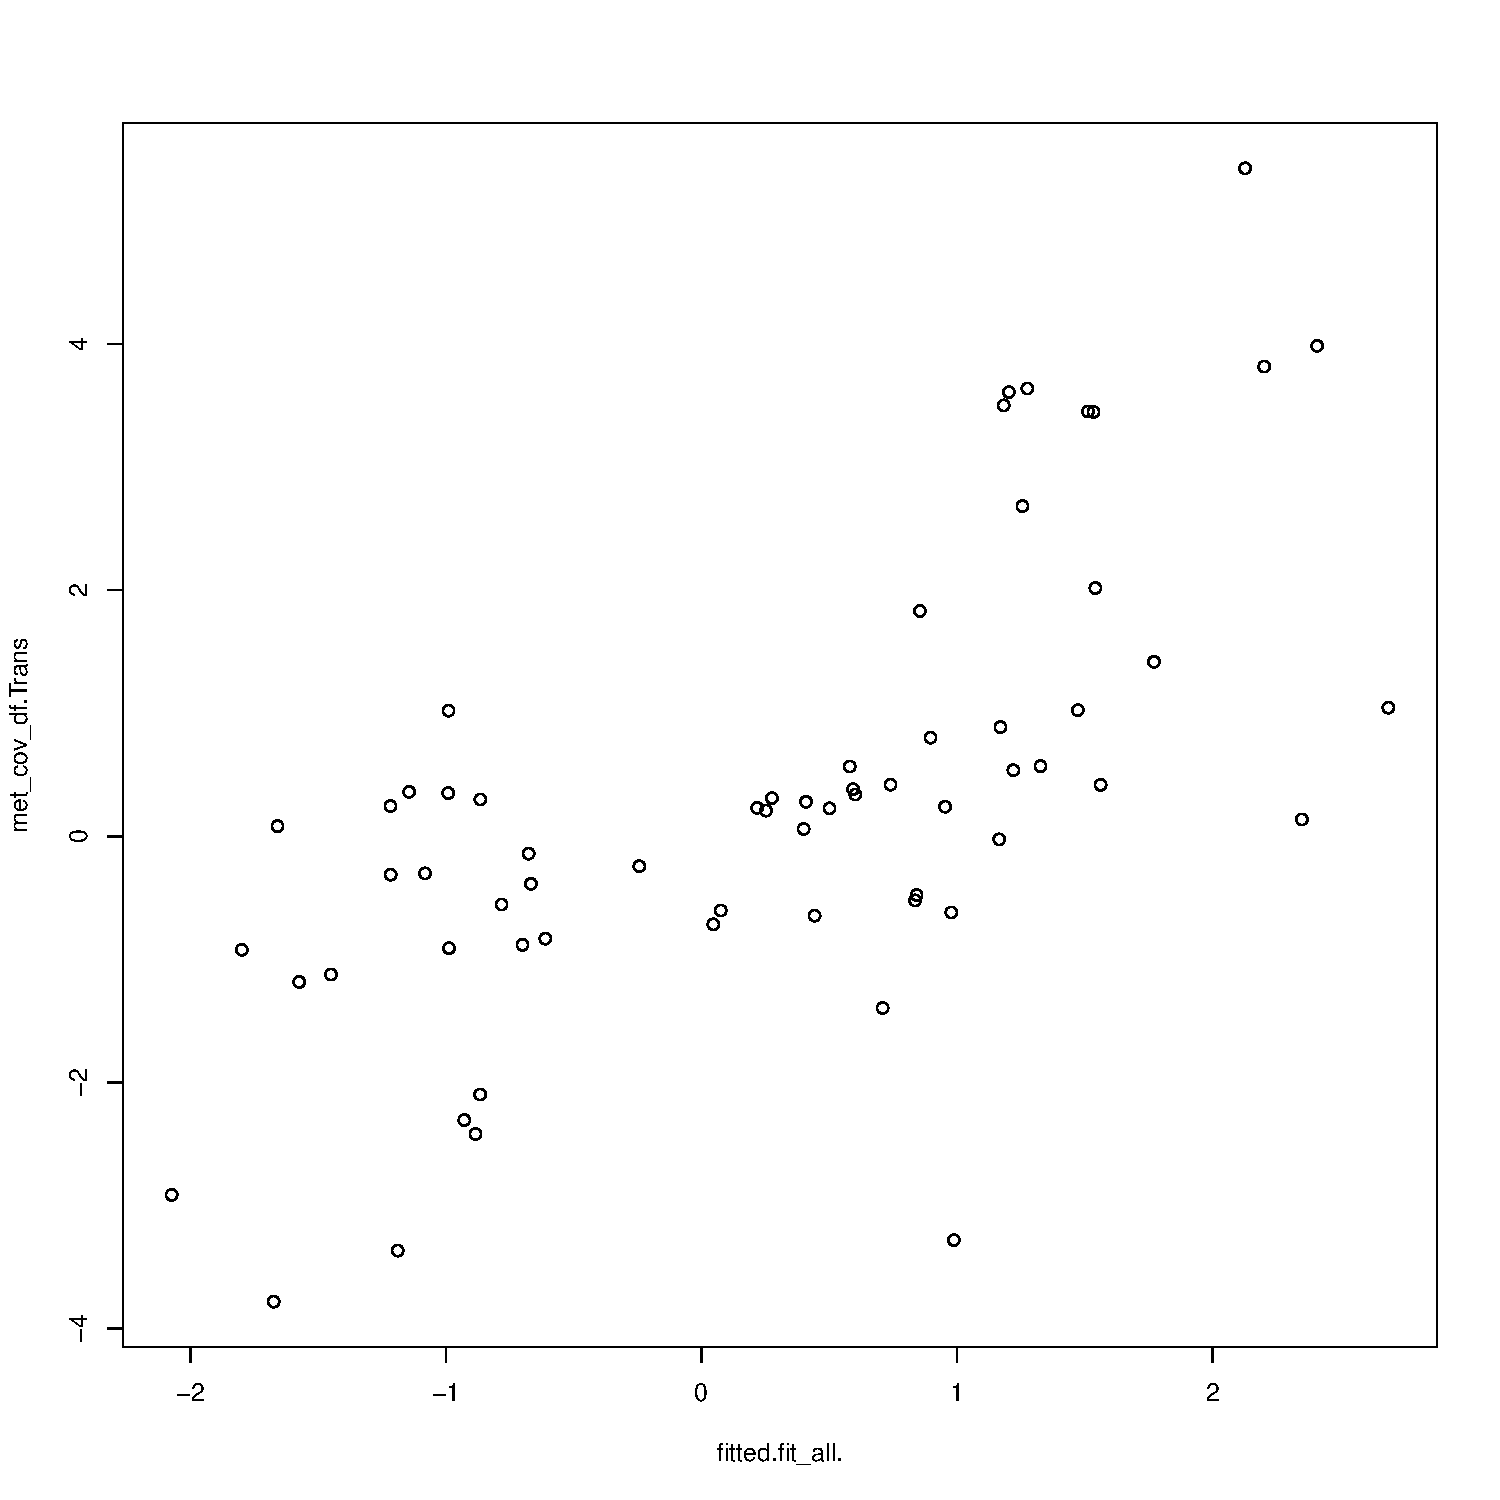
\includegraphics[width=.9\linewidth]{figure/minimal-heat_fitted_model-1} 
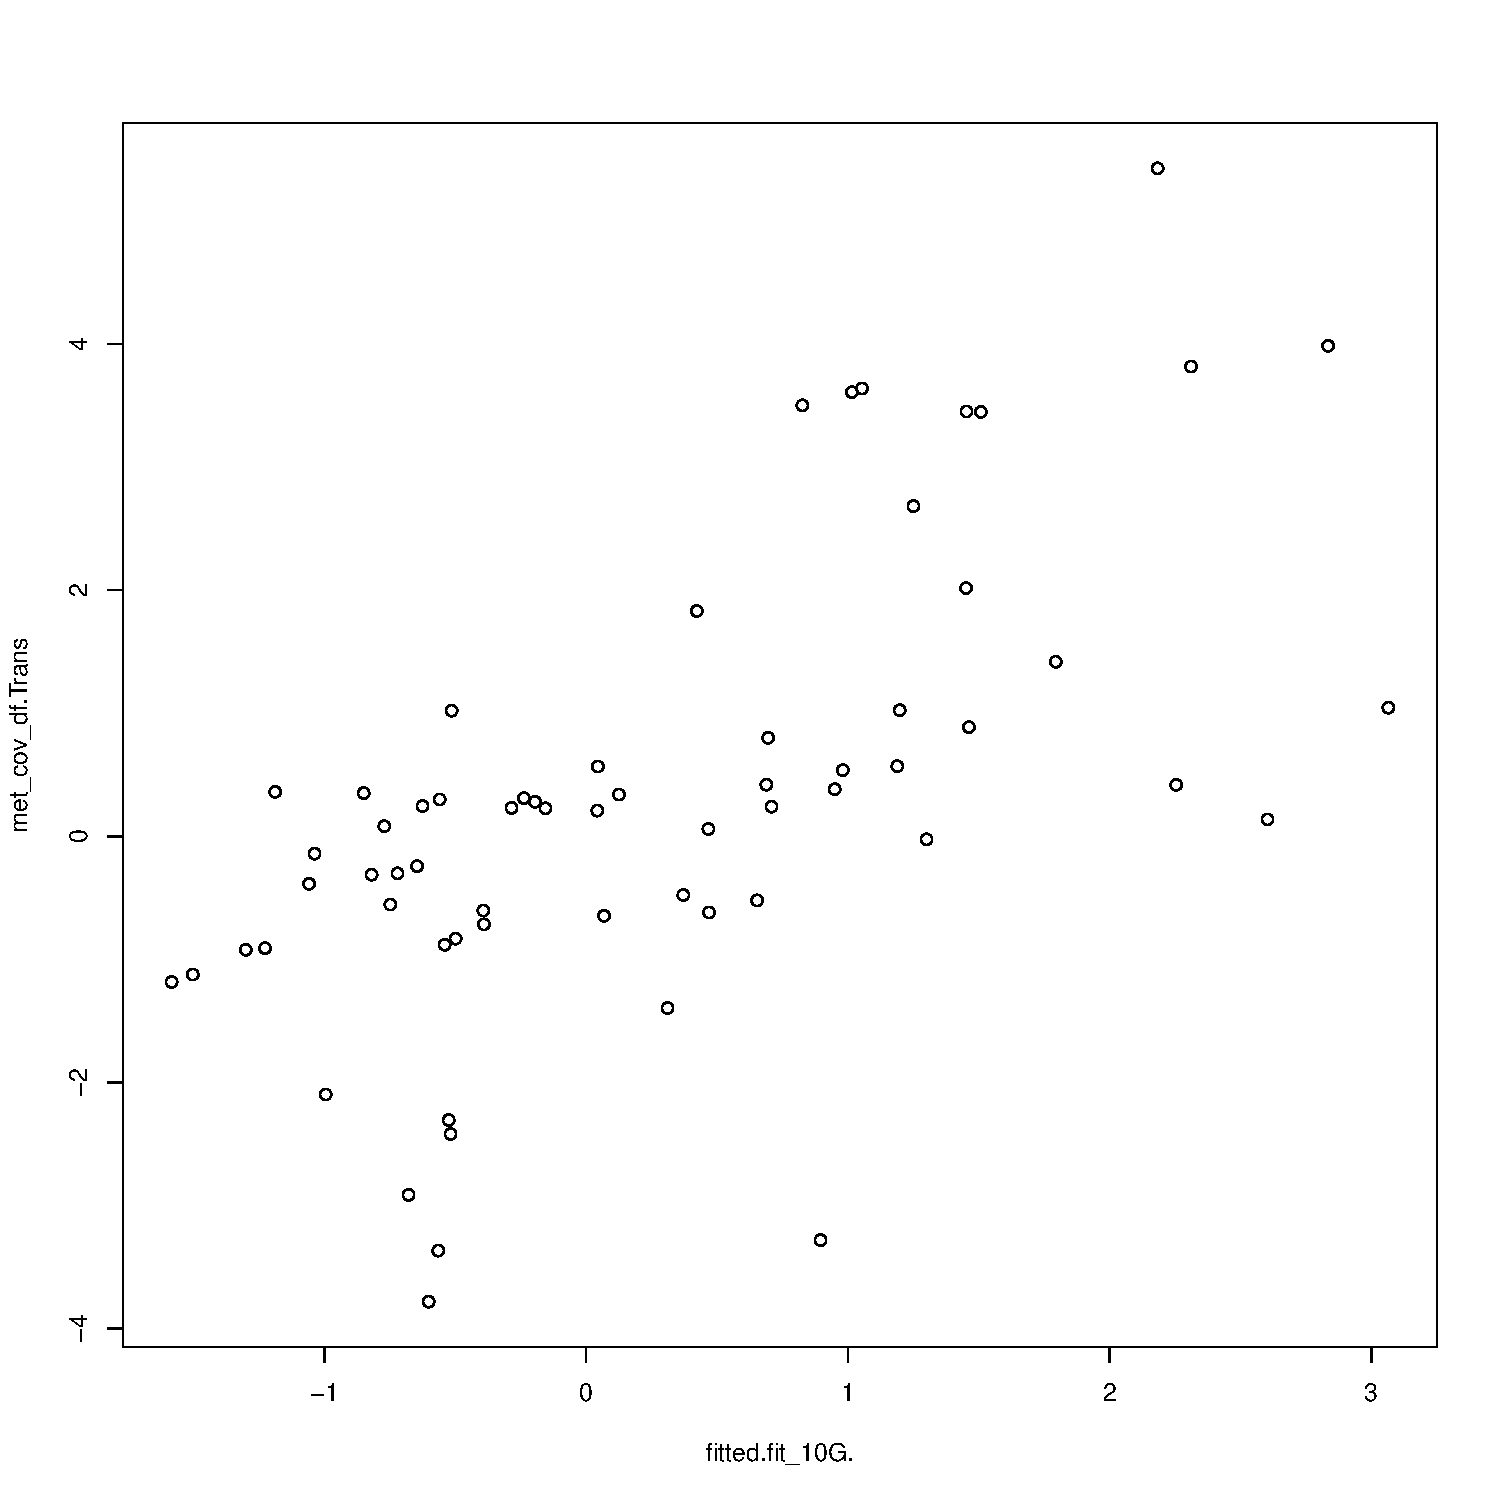
\includegraphics[width=.9\linewidth]{figure/minimal-heat_fitted_model-2} 
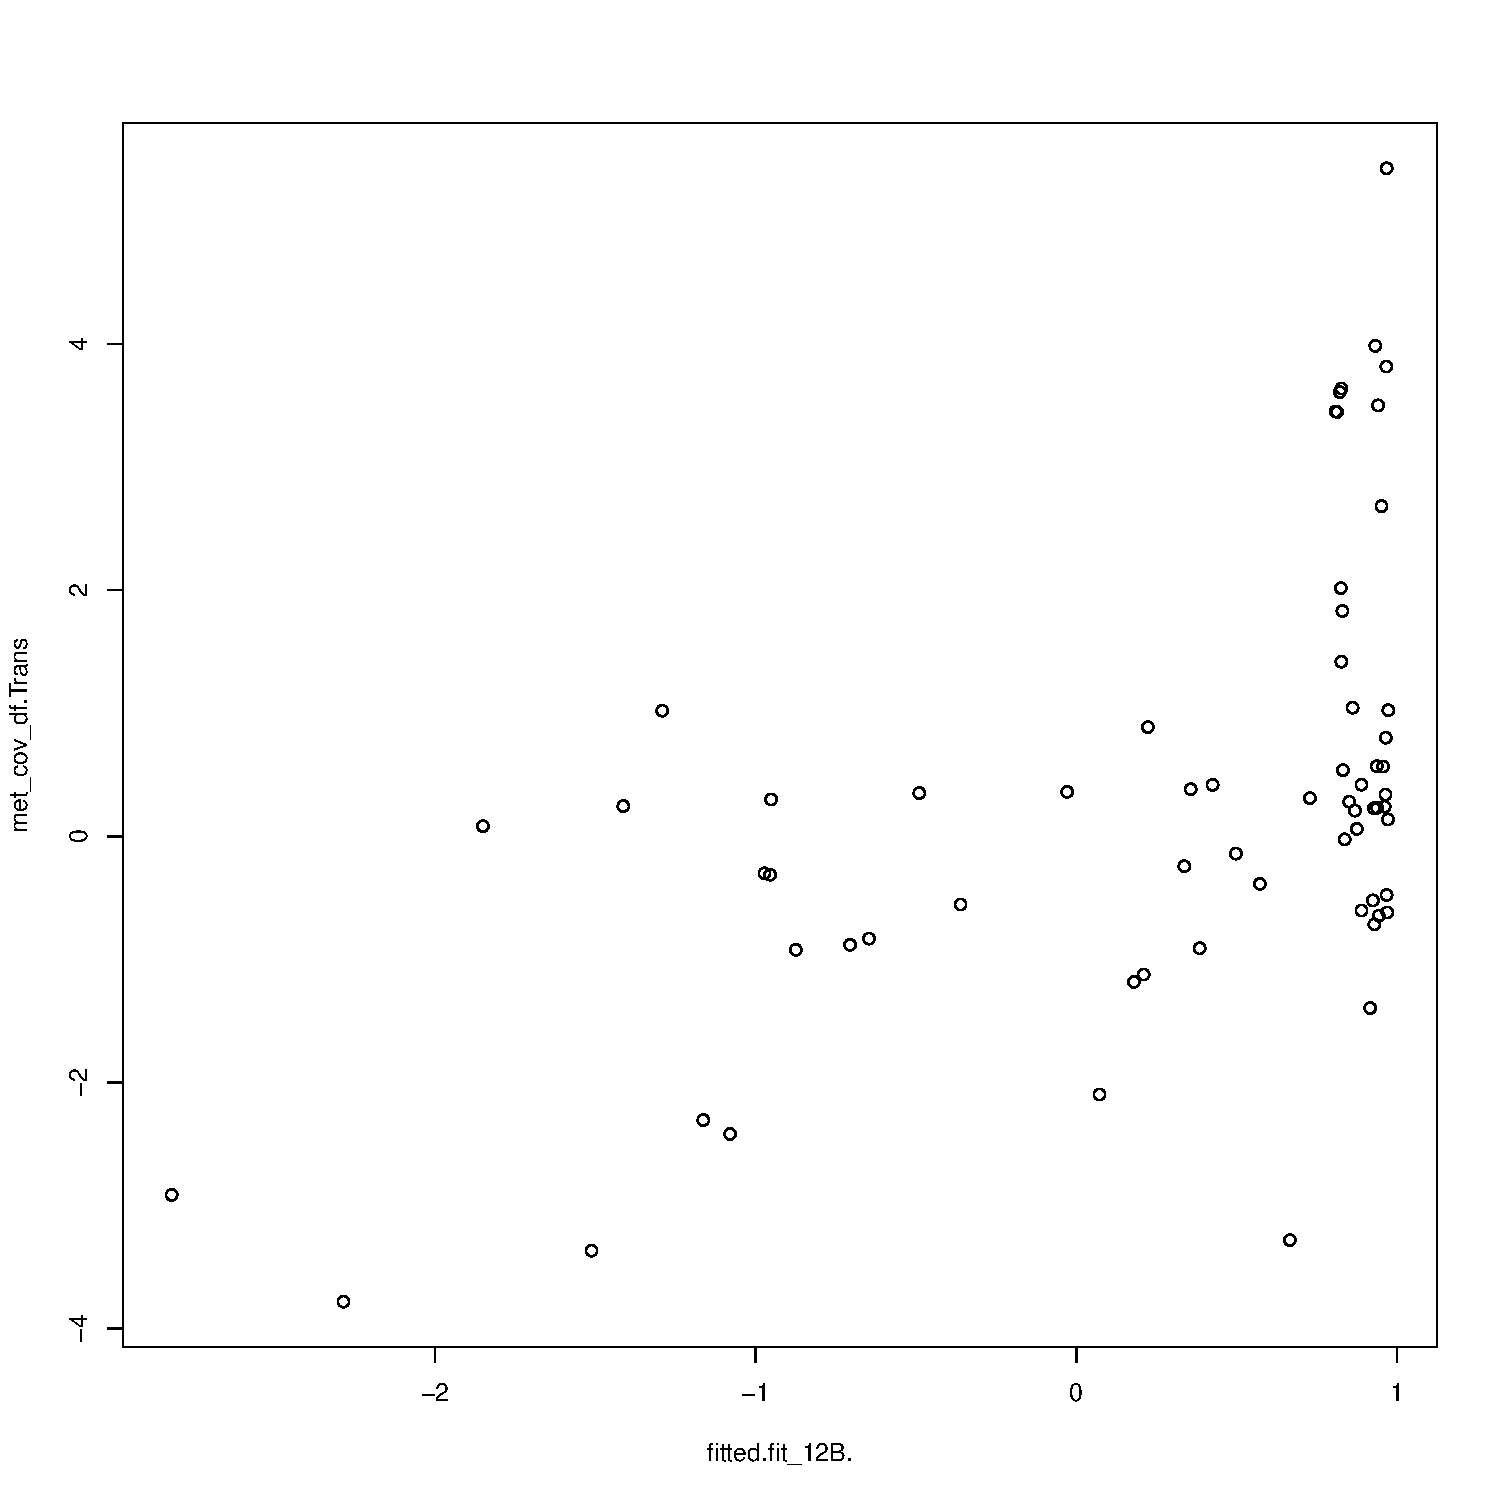
\includegraphics[width=.9\linewidth]{figure/minimal-heat_fitted_model-3} 
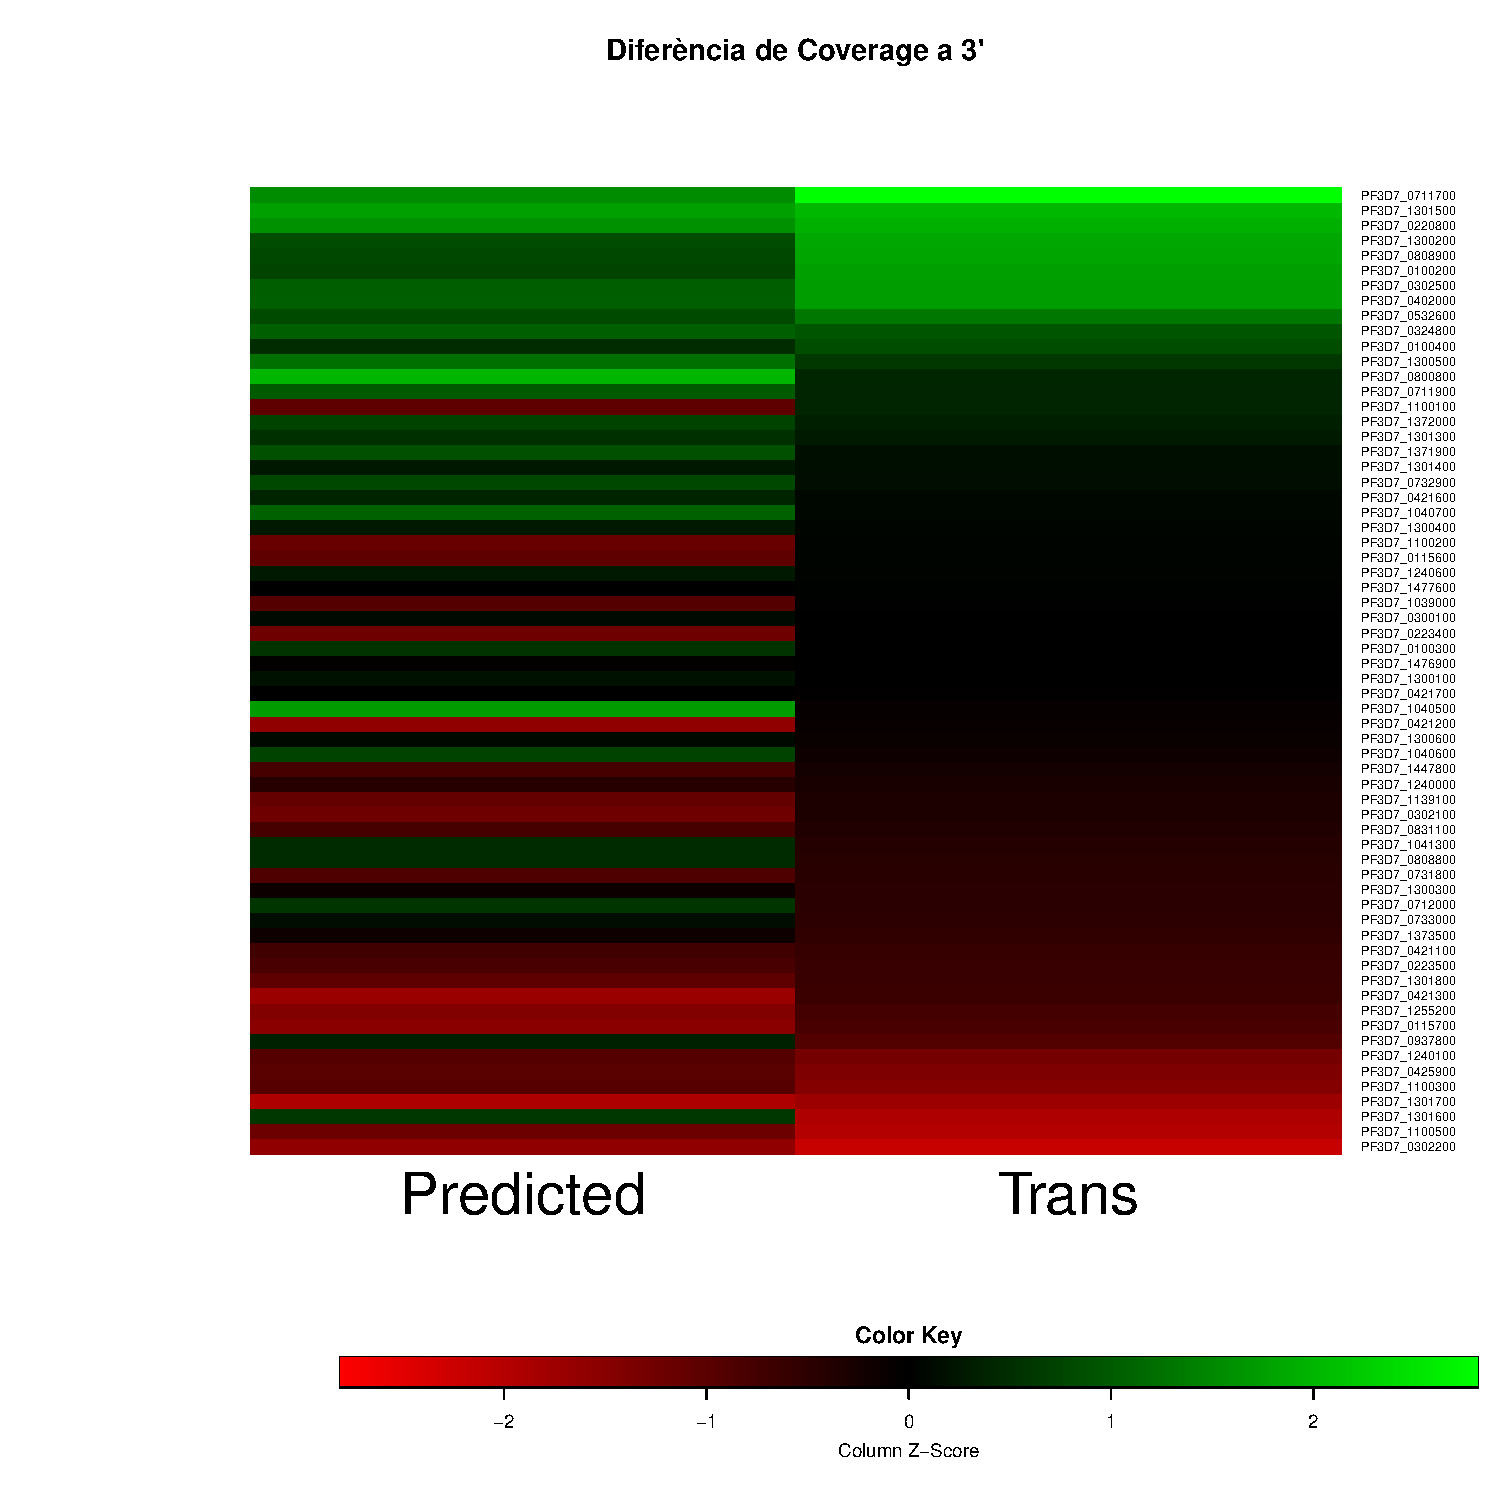
\includegraphics[width=.9\linewidth]{figure/minimal-heat_fitted_model-4} 

}



\end{knitrout}




\end{document}
